\chapter{Testing and Evaluation}
\label{chap:eval}
\lhead{\emph{Project Testing}}
%The goal of this chapter is an objective evaluation of the final system. The evaluation must be quantitative and not qualitative. You may perform qualitative evaluation but this should not form the basis of the main conclusions you derive from the evaluation. This evaluation, where possible, should be comparative, i.e. you should evaluate your system against a commercially available system and/or system detailed in a research publication. You should demonstrate operational testing of the project using real or contrived data sets to evaluate aspects of the project not encompassed in the software testing (e.g. quantify how well does your project achieved the overall goal). 
%\begin{itemize}
%    \item For software based projects this will include, but should not be limited to, evaluation of non-functional requirements.
%    \item For infrastructural projects this testing should include system/network KPI analysis.
%    \item For analysis based projects (ML, malware or other) this may include model evaluation or YARA rule validation, for example.
%    \item For management projects, where software testing or infrastructure testing may not be in scope, the test process for the system is expected to be more rigorous and well described than a project incorporating significant development work.
%\end{itemize} 
%
%Some suggested sections (the nature of this chapter should be discussed in detail with your term 2 supervisor):
%
%\section{Metrics}
%Identify and describe the metrics you used to evaluate your project. You should have identified some of these in the research phase report but will detail these as you progress through the design.
%
%\section{System Testing}
%Describe the experimental setup for each metric, and how you obtained the measurements. Describe the inputs for each experiment
%
%\section{Results}
%Summarise the output data, and the statistical or other techniques to deduce your results. Summarise your results, including tables or graphs as appropriate with a brief description of each. here possible, compare your results with other products/systems. Identify any possible threats to the validity of your results, and discuss each briefly here (you will discuss in more detail in the next chapter).
%
This chapter will go into more detail into how DynamiCrypt actually works. There will various code snippets present throughout this chapter. After an explanation of how parts of the system work tests will also be carried out. 

\section{The Beginning}
C++ is a compiled language and DynamiCrypt requires quite a few libraries to be present for linking. The command to compile DynamiCrypt is the following.
\begin{lstlisting}
g++ *.cpp -lboost_system -lpthread -lboost_thread -lboost_program_options -lcryptopp -lpistache -o DynamiCrypt
\end{lstlisting}

\begin{figure}[!h]
  \centering
      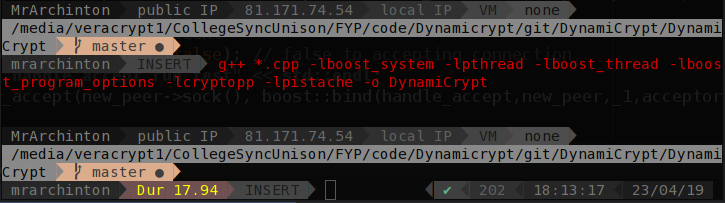
\includegraphics[width=1\textwidth]{Figures/b1.png}
  \caption[Compiling DynamiCrypt]{Compiling DynamiCrypt}
  \label{fig:b1}
\end{figure}
\FloatBarrier

Figure \ref{fig:b1} shows the result of the compilation and as you can see there are no errors or warnings present, this is an indication that the code is syntax correct and operations are performed for the correct data types.

Every program starts of with a main function. DynamiCrypt's main function is rather light, all it does is processes the command line arguments, creates a listening peer and creates the API server object.
To create an initial peer the already seen before code is used.
\begin{lstlisting}
ip::tcp::acceptor acceptor(service, ip::tcp::endpoint(ip::tcp::v4(), listen_port));
peer::ptr initial_peer = peer::new_(false);
acceptor.async_accept(initial_peer->sock(), boost::bind(handle_accept,initial_peer,_1, &acceptor));
\end{lstlisting}
Here an acceptor object is created this allows for the peer object to listen on a port on the localhost.
\begin{lstlisting}
peer::new_(false);
\end{lstlisting}
Is used to notify the peer object that this peer will be waiting for a connection.
\begin{lstlisting}
void handle_accept(peer::ptr peer, const boost::system::error_code & err, ip::tcp::acceptor* acceptor) {
    peer->start("",""); // starts current client
    // creates and listens for new client
    peer::ptr new_peer = peer::new_(false); // false to accepting connection
    //std::cout << "handle_accept run test" << std::endl;
    acceptor->async_accept(new_peer->sock(), boost::bind(handle_accept,new_peer,_1,acceptor)); // this 
}
\end{lstlisting}
The above function is called when the asynchronous connect object receives an external tcp request. The start method is called on the current peer followed by a creation of a new peer which will start listening for the next connection. This way there is always only one peer waiting for new connections. 

Because of how Boost manages asynchronous programming by using a service object to manage threads as well as using the proactor design pattern where asynchronous operations can occur using only one thread. However because DynamiCrypt is operation heavy when it comes to synchronisation I have used both threads and the proactor approach, this way when an asynchronous operation is about to take place Boost will choose a random available thread for it to run on. 
For this reason there are a few operations taking place in the main.cpp file to set all of this up.
\begin{lstlisting}
boost::thread_group threads;

start_listen(4);

void start_listen(int thread_count) {
    for ( int i = 0; i < thread_count; ++i)
        threads.create_thread( listen_thread);
}

void listen_thread() {
    service.run();
}

}
\end{lstlisting}
A group of threads variable is allocated, then the start listen function is called in the main function, this function creates four threads in this case and executes the service.run() function in each thread. This just executes boost asynchronous handler on each of the four threads. 

Finally to ensure a clean exit without leaving any zombie processes the main function will wait for all the threads to finish their execution.
\begin{lstlisting}
threads.join_all();
\end{lstlisting}

The API server is a bit more straight forward since the threads and asynchronous operations are more hidden away from the user by the Pistache library. 
\begin{lstlisting}
api_service_data_handler.set_address_and_port_of_sync("127.0.0.1", listen_port);
APIServer api_server(api_port);
\end{lstlisting}
The first line here sets the address of the sync-server and the port on which it is listening on as this information will be shared with the NodeJs app later. 
The actual creation of the API is simply calling the constructor with a port number.

The API and the sync-server require each other for operation, however it would be confusing if both were explained at the same time therefore the API will be covered initially followed by the sync-server.

\section{API}
The constructor of the API server creates the variables needed for the server and ofloads it to the APIservice object.
\begin{lstlisting}
APIServer::APIServer(int port_number) {
    Pistache::Port port(port_number);
    int thr = 2;
    Pistache::Address addr(Pistache::Ipv4::any(), port);
    //cout << "Cores = " << hardware_concurrency() << endl;
    std::cout << "API Using " << thr << " threads" << std::endl;
    API_service api(addr);
    api.init(thr);
    api.start();
    api.shutdown();
}
\end{lstlisting}
For the API two threads were defined as this is enough to handle multiple clients.
The threads are created as follows.
\begin{lstlisting}
void API_service::init(size_t thr = 2) {
    auto opts = Pistache::Http::Endpoint::options()
        .threads(thr)
        .flags(Pistache::Tcp::Options::InstallSignalHandler);
    httpEndpoint->init(opts);
    createDescription();
}
\end{lstlisting}
Pistache is a much more high level library than Boost therefore for the setup I mostly followed the examples they have in their GitHub repository.
\begin{lstlisting}
void API_service::start() {
    router.initFromDescription(desc);
    httpEndpoint->setHandler(router.handler());
    httpEndpoint->serve();
}
\end{lstlisting}
start() sets up the description which in Pistache's case is the information about all the routes available, some licensing and API info.  

Here is a small extract from the function that creates the description
\begin{lstlisting}
void API_service::createDescription() {
    desc
        .info()
        .license("Apache", "http://www.apache.org/licenses/LICENSE-2.0");

    auto backendErrorResponse =
        desc.response(Pistache::Http::Code::Internal_Server_Error, "An error occured with the backend");

    desc
        .schemes(Pistache::Rest::Scheme::Http)
        .basePath("/v1")
        .produces(MIME(Application, Json))
        .consumes(MIME(Application, Json));

    auto versionPath = desc.path("/v1");

    auto path = versionPath.path("/options");

    path
        .route(desc.get("/test-ok"))
        .bind(&API_service::route_test, this)
        .produces(MIME(Application, Json), MIME(Application, Xml))
        .response(Pistache::Http::Code::Ok, "ok");
    
    path
        .route(desc.post("/init"), "Initiate Communication")
        .bind(&API_service::initial, this)
        .produces(MIME(Application, Json))
        .consumes(MIME(Application, Json))
        .response(Pistache::Http::Code::Ok, "Initial request")
        .response(backendErrorResponse);
\end{lstlisting}
The path is built by firstly specifying the version of the API this way it is possible to support legacy code using you old API. Next I decided to put all the DynamiCrypt operations preceded by /options this way in the future if the API can be expanded to do other things like maybe formatting / encoding data. Next is the actual routes used by the DynamiCrypt API. The first one is /test-ok a GET route, this is handy if you want to check if the API is up and running. To access this route you would send a get request to this for example 127.0.0.1:9081/v1/options/test-ok/. This simple route will just return "ok" as can be seen when a curl get request is being made as can be seen in figure \ref{fig:b2}.

\begin{figure}[!h]
  \centering
      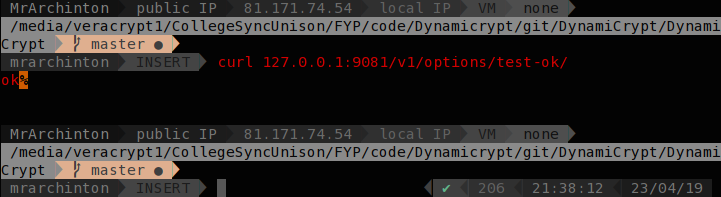
\includegraphics[width=1\textwidth]{Figures/b2.png}
  \caption[127.0.0.1:9081/v1/options/test-ok/]{127.0.0.1:9081/v1/options/test-ok/}
  \label{fig:b2}
\end{figure}
\FloatBarrier

The list of all routes currently available in the API and a brief description are as follows.
\begin{lstlisting}
/v1/options/test-ok         GET
// test if API is up
/v1/options/init            POST
// Initial request
/v1/options/init_config     POST
// Initial Config
/v1/options/sync            POST
// Begin Sync
/v1/options/status          POST
// check if connected to tpm ok
/v1/options/encrypt         POST
// encrypt / decrypt data
/v1/options/exit            POST
// delete tpm and data associated with the app using the API
/v1/options/:rest           POST
// custom 404
\end{lstlisting}

Every post route is handled by a specific function.
\begin{lstlisting}
 path
        .route(desc.post("/init"), "Initiate Communication")
        .bind(&API_service::initial, this)
        .produces(MIME(Application, Json))
        .consumes(MIME(Application, Json))
        .response(Pistache::Http::Code::Ok, "Initial request")
        .response(backendErrorResponse);
\end{lstlisting}

In this case every time the init route is called the initial() function handles it and produces its own response. Here is the initial function bellow.

\begin{lstlisting}
void API_service::initial(const Pistache::Rest::Request& request, Pistache::Http::ResponseWriter response) {
    rapidjson::Document document;
    // make into json object
    char * jsonBody = new char [request.body().length()+1];
    strcpy (jsonBody, request.body().c_str());
    document.Parse(jsonBody);
    
    std::string service_name;
    int data_ok = 1;

    if(document.HasMember("service_name")){
        if(document["service_name"].IsString()){
            service_name = document["service_name"].GetString();
        }
        else{
            data_ok = 0;
        }
    }
    else{
        data_ok = 0;
    }
    
    std::string respond_service_name;
    rapidjson::StringBuffer buffera;
    rapidjson::Writer<rapidjson::StringBuffer> writera(buffera);
    
    if(data_ok){
        respond_service_name = api_service_data_handler.new_service(service_name);
        writera.StartObject(); 
        writera.Key("service_name");                
        writera.String(respond_service_name.c_str(), respond_service_name.length());
        writera.Key("address_of_this_tpm");                
        writera.String(api_service_data_handler.get_sync_address().c_str(), api_service_data_handler.get_sync_address().length());
        writera.Key("port_of_this_tpm");
        writera.Uint(api_service_data_handler.get_sync_port());
        writera.EndObject();
        
    }
    
    else{//error with request
        writera.StartObject(); 
        writera.Key("error");                
        writera.String("invalid request");
        writera.EndObject();
    }
    
    response.send(Pistache::Http::Code::Ok, buffera.GetString());
}
\end{lstlisting}

Similar to NodeJs each of these handlers have a reference to a request and response object.
For extracting JSON data the RapidJson library is used, it is also used for creating JSON data.
The API interacts with the 
\begin{lstlisting}
api_service_data_handler
\end{lstlisting} 
object for managing the services.

It will take too long to go through all of the routes and how they function so a more basic explanation will suffice. I would recommend watching my demo video here https://www.youtube.com/watch?v=LsR4XsGrDCY&feature=youtu.be 
on YouTube as it would be easier to understand.

Initially the NodeJs apps must register with the API this unfortunately turned out to be a multi step process however it is necessary since the API needs data from both of the Apps that wish to use DynamiCrypt.

\begin{figure}[!h]
  \centering
      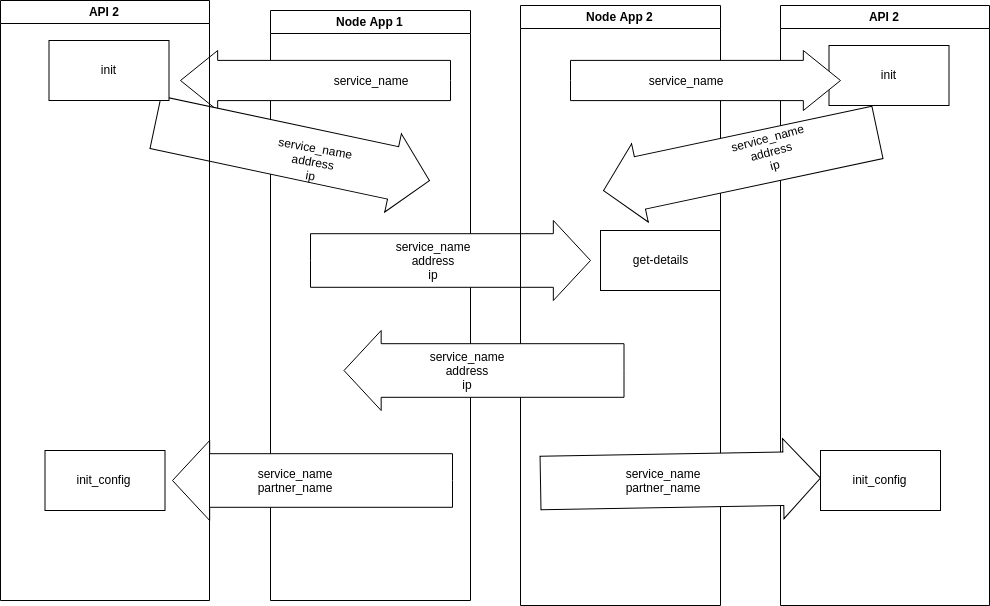
\includegraphics[width=1\textwidth]{Figures/connect_code_flow.png}
  \caption[How Node Apps register with the API]{How Node Apps register with the API}
  \label{fig:b3}
\end{figure}
\FloatBarrier

Figure \ref{fig:b3} is a call flow diagram of how the NodeJS apps register themselves with the API.
The same can be demonstrated by using Wireshark and listening on localhost. The filters I used are (tcp.port == 9081) && http since I only want to see POST requests for the API running on port 9081 since the POST requests for the other API are identical so there is no point in showing it twice.

\begin{figure}[!h]
  \centering
      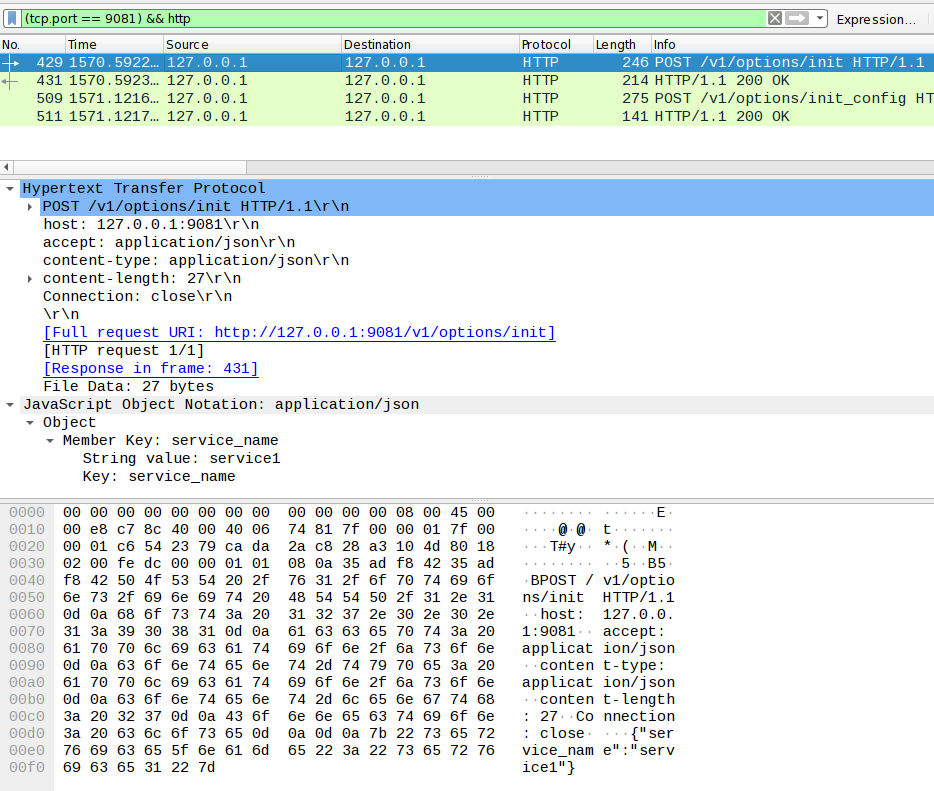
\includegraphics[width=1\textwidth]{Figures/b4.png}
  \caption[POST request to init]{POST request to init}
  \label{fig:b4}
\end{figure}
\FloatBarrier
Figure \ref{fig:b4} shows how the NodeJs App sent a POST request to the init route with its user service name. 

\begin{figure}[!h]
  \centering
      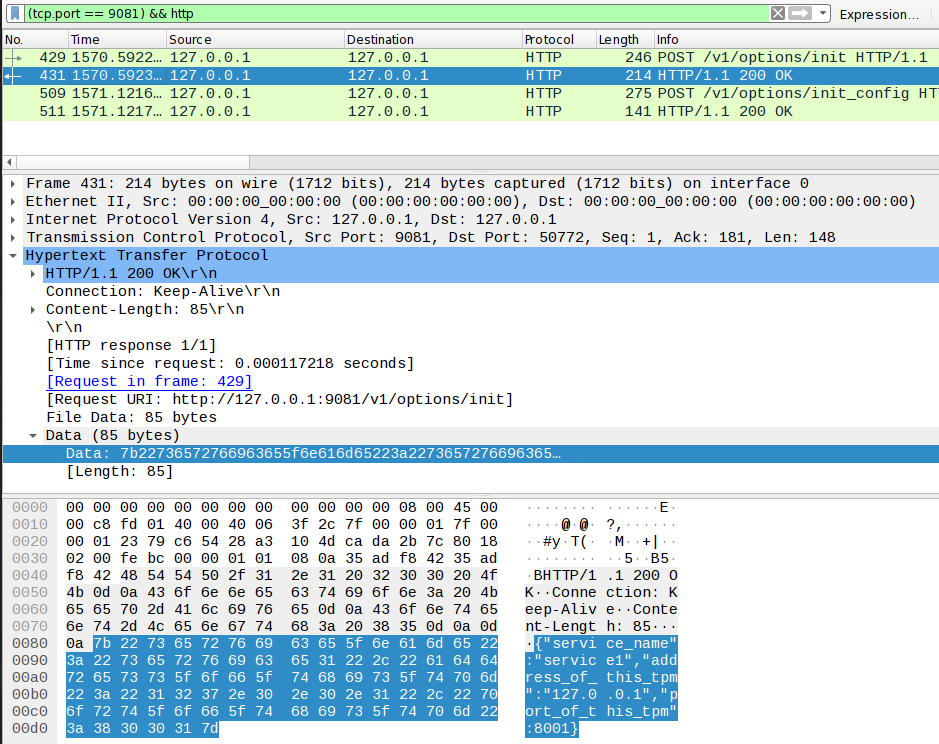
\includegraphics[width=1\textwidth]{Figures/b5.png}
  \caption[API response]{API response}
  \label{fig:b5}
\end{figure}
\FloatBarrier
Figure \ref{fig:b5} shows how the APIs reply to the previous post request with the service name the API wants the NodeJS App to use, the port of the sync-server and the address of the sync-server.
After this the Node App would make a request to the other Node App for the get details route to exchange information. This can also be acquired with Wireshark by changing a filter as seen in figure \ref{fig:b8}.
\begin{figure}[!h]
  \centering
      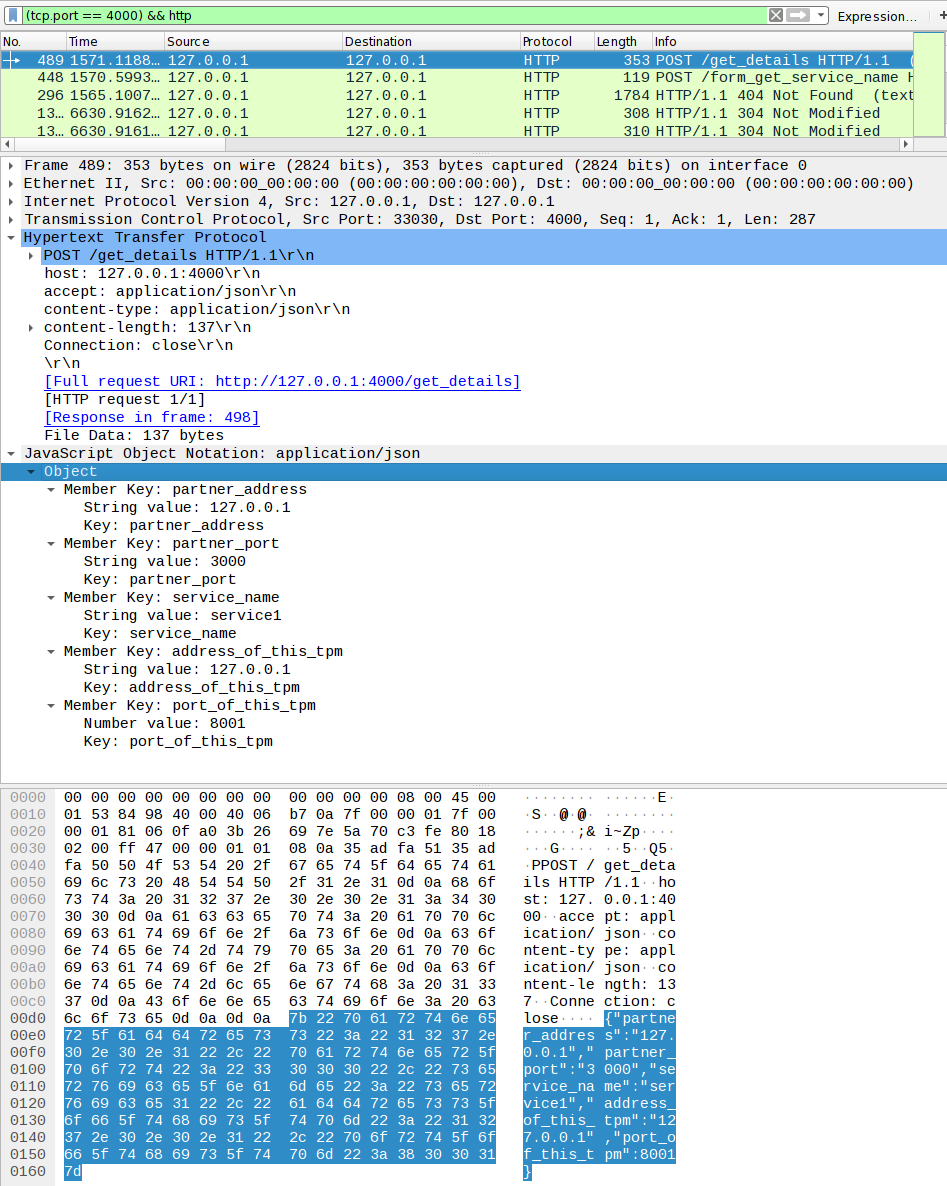
\includegraphics[width=1\textwidth]{Figures/b8.png}
  \caption[POST request to other NodeJs app's get details route]{POST request to other NodeJs app's get details route}
  \label{fig:b8}
\end{figure}
\FloatBarrier


\begin{figure}[!h]
  \centering
      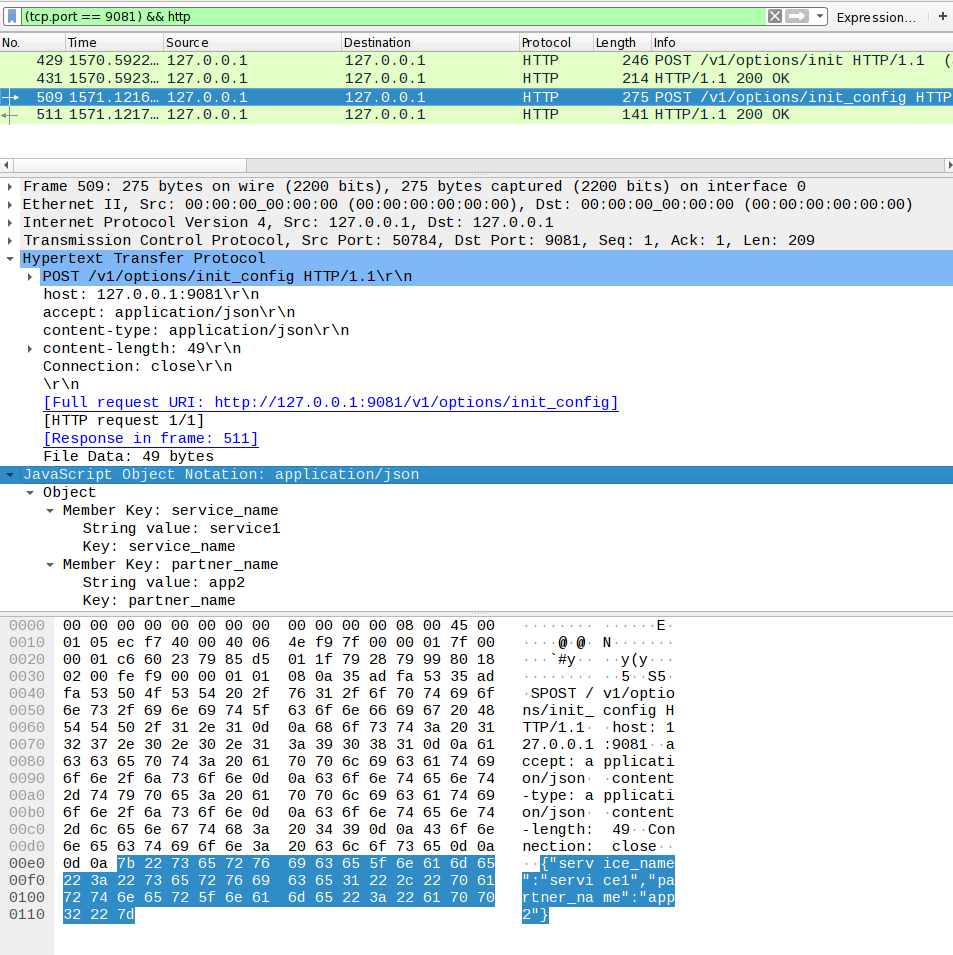
\includegraphics[width=1\textwidth]{Figures/b6.png}
  \caption[POST request to init config]{POST request to init config}
  \label{fig:b6}
\end{figure}
\FloatBarrier
Figure \ref{fig:b6} shows how the NodeJs app updates the API with the service name of the other NodeJs app in this case it is called partner name.

\begin{figure}[!h]
  \centering
      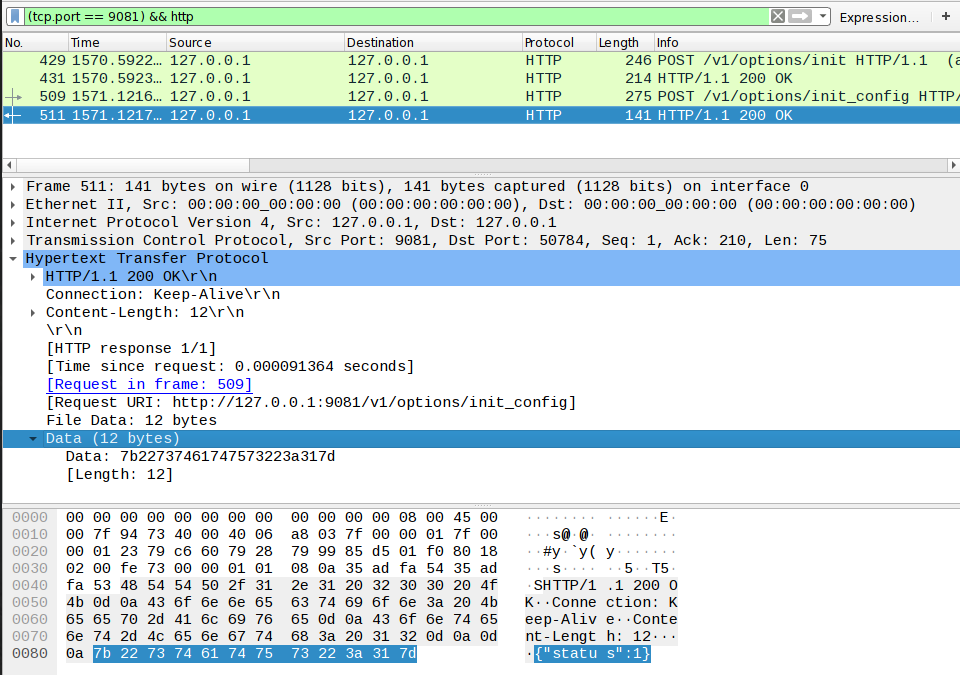
\includegraphics[width=1\textwidth]{Figures/b7.png}
  \caption[API response]{API response}
  \label{fig:b7}
\end{figure}
\FloatBarrier
Figure \ref{fig:b7} shows the APIs reply to the previous post request with a status 1 which means everything is OK and the update was successfully made.
Now the two NodeJs apps are fully registered with the API. The next step is to tell the API to tell the sync-server to start synchronising so that the Apps can send messages to each other using dynamic encryption.
For this to occur one of the Apps must simply call the sync route of the API.

\begin{figure}[!h]
  \centering
      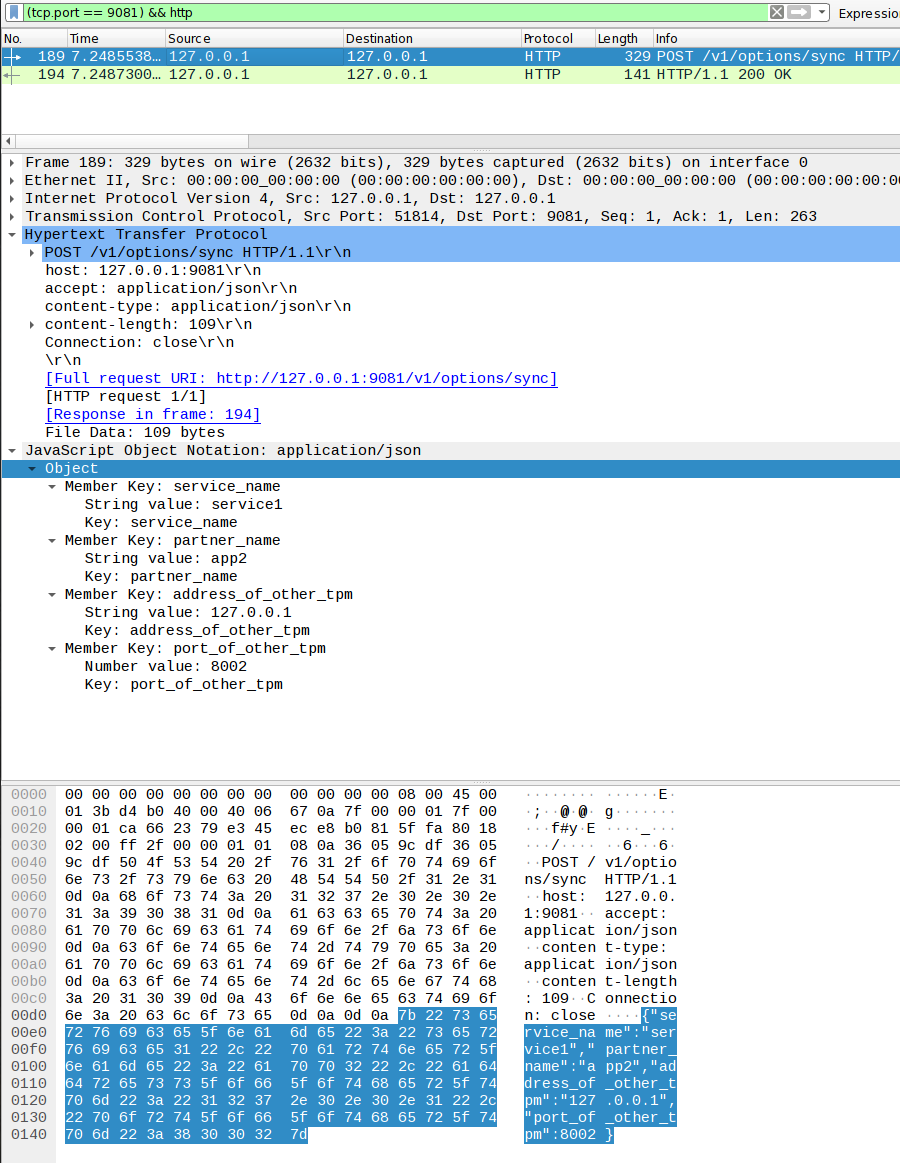
\includegraphics[width=1\textwidth]{Figures/b9.png}
  \caption[POST request to sync]{POST request to sync}
  \label{fig:b9}
\end{figure}
\FloatBarrier
Figure \ref{fig:b9} shows the sync route of the API is called. The Node App sends a lot of details this time including service name, partner name, the address and port of the sync-server that is used by the other API that the other NodeJs App communicates with. This is because it is calling a different function outside of the api service data handler object. This time a function from the definitions.cpp is called.
\begin{lstlisting}
int begin_sync(std::string address, int port, std::string service_name, std::string partner_name){
    try{
        peer::ptr initiating_peer = peer::new_(true, address, port);
        initiating_peer->start(service_name, partner_name);
    }
    catch(std::exception& e){
        return 0;
    }
    return 1;
}
\end{lstlisting} 
Here a new peer is created of connecting type instead of listening type like we looked at last time. This peer will try to connect to the sync-server at the address and port the Node App sent it.

\begin{figure}[!h]
  \centering
      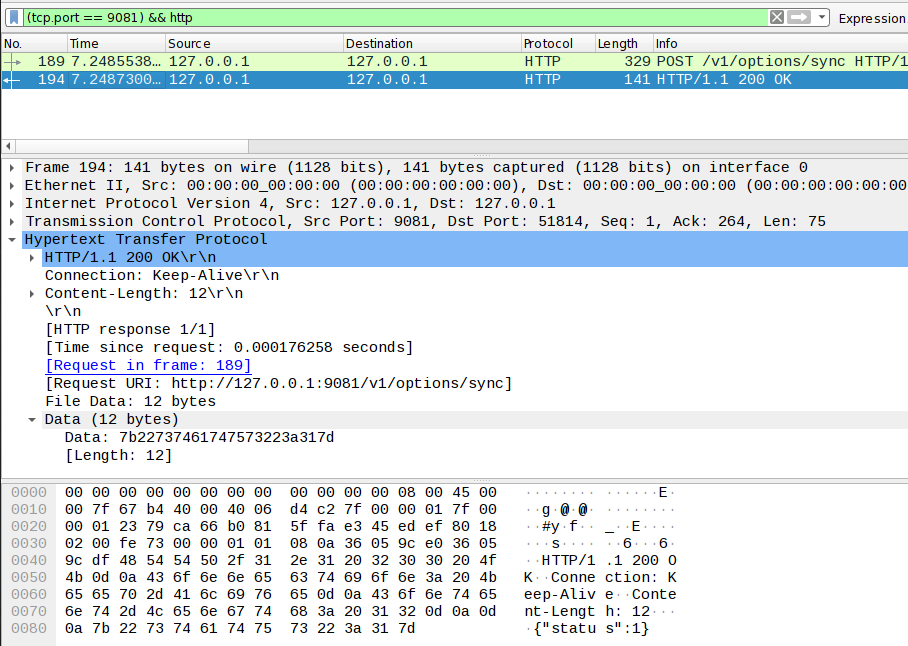
\includegraphics[width=1\textwidth]{Figures/b10.png}
  \caption[API response]{API response}
  \label{fig:b10}
\end{figure}
\FloatBarrier
Figure \ref{fig:b10} shows the APIs reply to the previous post request with a status 1 which means the request was processed successfully however this does not mean that the sync-server connected to the other sync-server correctly this is because of the asynchronous nature of the sync-server it is impossible to get the result of the connection. Therefore the NodeJs app should query the API to see if the connection was successful and if the two sync-servers are currently syncing this is done by calling the status route in the API and providing the service name. if the status returned is 1 then the two sync-servers are currently synchronising, if the status is 0 then they failed to connect or some other error occurred.

\textbf{Encryption / Decryption}

Now the NodeJs apps can send messages to the API to be encrypted.
How encryption works is it selects the appropriate key from the key store based on the mode provided.
The key store looks like this.
\begin{lstlisting}
struct key_store {
    std::string key;
    int uses;
};

struct API_data {
    std::string service_name_;
    std::string service_name_partner_;
    std::vector<key_store> keys_;
};
\end{lstlisting} 
This is an inner struct inside the 
\begin{lstlisting}
API_service_data_handler
\end{lstlisting} 
class which contains a vector of API data objects.

Currently DynamiCrypt supports two encryption methods. Encryption mode 1 will simply use the latest key avaiable in the keystore, this mode is handy if you want the fastest mode of encryption available.
For encryption mode 1, 
\begin{lstlisting}
if(mode == 1){
                //check for any latest key 
                if(api_data->keys_.size() == 0){
                    return DYNAMICRYPT_API_WAIT;
                }else{
                    string_key = api_data->keys_.back().key;
                    api_data->keys_.back().uses ++;
                    if(PRINT_API_CRYPT_MESSAGES){
                        std::cout << "got key like this " << string_key << std::endl;
                        std::cout << "key was used " << api_data->keys_.back().uses << " times" << std::endl;
                    }
                }
            
            }
\end{lstlisting} 
The appropriate api data object is selected referring to the service that called the API.
The size of the key store is initially checked to see if it contains any keys, if not then the API will tell the Node App to wait. The node app can then query the API again and again for encryption or just use a timeout and wait for 100 milliseconds or so. 
If there is keys in the key store then the last key that was entered is used for encryption. The uses count of this particular key is also increased, the uses count doesn't really matter for mode 1 but will matter for mode 2 and future modes that are not implemented yet. 

Encryption mode 2 would be the more secure one as only keys that have 0 uses are picked this way each message would be encrypted using its own unique key.
\begin{lstlisting}
else if (mode == 2){
                if(api_data->keys_.size() == 0){
                    return DYNAMICRYPT_API_WAIT;
                }
                else{
                    int attempts_to_find_key = 0; //search max_attempts_to_decrypt times for the key since decrypt will only search for max_attempts_to_decrypt times too
                    int found_key = 0;
                    for(int number_of_keys = api_data->keys_.size()-1; number_of_keys >= 0; number_of_keys --){
                        if(attempts_to_find_key == max_attempts_to_decrypt){
                            break;
                        }
                        attempts_to_find_key ++;
                        if(api_data->keys_.at(number_of_keys).uses == 0){
                            string_key = api_data->keys_.at(number_of_keys).key;
                            api_data->keys_.at(number_of_keys).uses++;
                            if(PRINT_API_CRYPT_MESSAGES){
                                std::cout << "got key like this " << string_key << std::endl;
                                std::cout << "key was used " << api_data->keys_.at(number_of_keys).uses << " times" << std::endl;
                            }
                            found_key = 1;
                            break;
                        }
                    }
                    if(!found_key){
                        return DYNAMICRYPT_API_WAIT;
                    }
                }
            }
\end{lstlisting} 
This mode is a little bit more involved then the simple get latest key. The Basic premise here is to find a suitable key that has 0 uses. This key is found by working back from the latest key down the vector until either a key is found, either the number of keys runs out or the search limit is reached. in this case the search limit is defined at 10 and stored at this variable.
\begin{lstlisting}
max_attempts_to_decrypt
\end{lstlisting} 
This means that in order to find a key provided the key store is longer than 10 the search will max out at 10 elements from the latest. 
This limit is set not so much for encryption but rather the decryption, this is because if there was no limit the encryption algorithm might choose a key that is say 200 keys away from the latest, the decryption algorithm will then have a heck of a time trying to find that correct key to use. 
And just like before if an appropriate key is not found the API will tell the Node App to wait.

After these two algorithms find the appropriate key the next step is to encrypt the data.
\begin{lstlisting}
CryptoPP::byte key[ CryptoPP::AES::MAX_KEYLENGTH ];
gen_key(string_key,key);
std::string for_encode = encrypt(message, key, iv);
\end{lstlisting} 
Earlier I said that the key generated by the tree parity machines will be used to encrypt the message. This is technically not true since that key is actually used to generate the actual key used for encryption. This is because the key generated by the tree parity machines is too long for AES-256 encryption therefore the gen key function generates an appropriate size key without loosing any data, this means that it does not simply cut of the rest of the key that's longer than 32 bytes needed for AES-256. Here is a snippet from that function.
\begin{lstlisting}
void API_service_data_handler::gen_key(std::string string_key, CryptoPP::byte* key){
    if(string_key.length() > CryptoPP::AES::MAX_KEYLENGTH){
            int count_first = 0;
            int count_last = string_key.length() -1;
            int number_of_operations = count_last - CryptoPP::AES::MAX_KEYLENGTH;
            for(int i = 0; i< number_of_operations; i++){
                string_key[count_first] = string_key.at(count_first) + string_key.at(count_last);
                if(count_first == CryptoPP::AES::MAX_KEYLENGTH){
                    count_first = 0;
                }
                count_first ++;
                count_last --;
            }
        }
        
        int string_count = 0;
        for(int i=0; i<CryptoPP::AES::MAX_KEYLENGTH; i++){
            if(string_count == string_key.length() -1){
                string_count = 0;
            }
            key[i] = string_key.at(string_count);
            string_count ++;
        } 
\end{lstlisting} 

After encrypting the data, the ciphertext is then encoded with base 64 encoding. Encoding is necessary because random bytes tend to mess up the structure of the JSON object.
\begin{lstlisting}
std::string encoded = encode_base64(for_encode);
output = encoded;
\end{lstlisting} 

Finally when sending the ciphertext to the node app the API also generates a hash specifically SHA 256 of the original plaintext. this will help the API to determine if the message was decrypted successfully by comparing hashes. Hashes are one way function so it is save to create a hash of the plaintext. The node app would then essentially just forward the ciphertext and the hash to the other node app for decrypting.

Decryption has algorithms specific for each mode therefore decryption mode 1 will directly be capable of decrypting encryption mode 1 and so on. The decryption is a potentially much more operation heavy operation that encryption. This is because it takes a guess at the key then tries to decrypt it and if that fails takes a guess at another key. This might seen pretty bad but from testing normally it only takes one to three decryption attempts to decrypt the key since the most likely key would be the latest one.

The decryption section of the code initially decodes the data from base 64 then that data is passed to the various decryption algorithms based on the mode.

For decryption mode 1
\begin{lstlisting}
if(mode == 1){
                if(api_data->keys_.size() == 0){
                    return DYNAMICRYPT_API_WAIT; // no keys in key ring shouldn't happen with decrypt if used properly
                }
                int number_of_keys = api_data->keys_.size()-1;  // maybe change to keys_.size()-1
                for(int decrypt_loop = 0; decrypt_loop<max_attempts_to_decrypt; decrypt_loop++){
                    //try last key first
                    std::string string_key = api_data->keys_.at(number_of_keys).key;
                    if(PRINT_API_CRYPT_MESSAGES){
                        std::cout << "trying to decrypt with key " << string_key << std::endl;
                        std::cout << "key was used " << api_data->keys_.at(number_of_keys).uses << " times" << std::endl;
                    }
                    CryptoPP::byte key[ CryptoPP::AES::MAX_KEYLENGTH ];
                    gen_key(string_key,key);

                    output = decrypt(decoded_message, key, iv);
                    if(!hash_with_sha_256(output).compare(hash)){ //decrypted successfully
                        api_data->keys_.at(number_of_keys).uses ++;
                        break;
                    }

                    if(number_of_keys == 0){
                        //output = "failed";
                        return DYNAMICRYPT_API_FAILED_DECRYPT;
                        break;
                    }

                    number_of_keys --;
                
                }
            }
\end{lstlisting} 
This checks if there are keys in the key ring this is not necessary since the tree parity machines generate the same keys at pretty much the same time but it is just in there as a sanity check or to catch some other strange errors. This is because for decryption the key is presumed to exist since that key was used to encrypt in the first place.

Since this is mode 1 we can simply try the latest key first then work down from there. Again how much further down you can go depends on the size of the key store and the limitation put in place to prevent traversing all the keys in case of an error or broken data.

Next the message is decrypted and hashed and the hash is compared to the hash sent by the node app. if the hashes match then the plaintext is returned if not the next key in line is tested.
If the hashes match the uses for the key is incremented this is important because you don't want this API using the same key for encryption as the other API if using mode 2. 
In the unlikely event that all the keys tried failed to decrypt the message a failure message will be sent to the node App, during testing I never have seen this scenario occur however it is likely to happen if you delay sending the encrypted data for decryption by quite some time like ten or more seconds since the key store will be filled up with new keys and the old key required for decryption will be pushed back past the limit. For this reason it is important for the node apps to send the ciphertext to the other node app as soon as possible.

For decrypting mode 2 quite a long algorithm is used. 
\begin{lstlisting}
else if (mode == 2){ // try keys with 0 uses first
                std::string string_key;
                if(api_data->keys_.size() == 0){
                    return DYNAMICRYPT_API_WAIT; // no keys in key ring shouldn't happen with decrypt if used properly
                }
                int has_skipped_keys = 0;
                int number_of_keys = api_data->keys_.size()-1;  // maybe change to keys_.size()-1
                
                //std::cout << "number_of_keys at start " << number_of_keys << std::endl;
                std::vector<int> skipped_keys;
                for(int decrypt_loop = 0; decrypt_loop<max_attempts_to_decrypt; decrypt_loop++){
                    //std::cout << "decrypt_loop at start " << decrypt_loop << std::endl;
                    if(number_of_keys == -1){ // needed because of the continue which could cause number_of_keys to be -1
                        break;
                    }
                    
                    if(api_data->keys_.at(number_of_keys).uses == 0){
                        
                        string_key = api_data->keys_.at(number_of_keys).key;
                        //std::cout << "key with 0 uses found " << string_key << std::endl;
                    }else{
                        skipped_keys.push_back(number_of_keys);
                        //std::cout << "skipping key at index " << number_of_keys << std::endl;
                        number_of_keys --;
                        has_skipped_keys = 1;
                        
                        continue;
                    }
                    
                    if(PRINT_API_CRYPT_MESSAGES){
                        std::cout << "trying to decrypt with key " << string_key << std::endl;
                        std::cout << "key was used " << api_data->keys_.at(number_of_keys).uses << " times" << std::endl;
                    }
                    CryptoPP::byte key[ CryptoPP::AES::MAX_KEYLENGTH ];
                    gen_key(string_key,key);

                    output = decrypt(decoded_message, key, iv);
                    if(!hash_with_sha_256(output).compare(hash)){ //decrypted successfully
                        api_data->keys_.at(number_of_keys).uses ++;
                        return output;
                    }

                    if(number_of_keys == 0){
                        break;
                    }

                    number_of_keys --;
                
                }
                //code runs here only if decryption was unsuccessful
                if(has_skipped_keys){ //check for skipped keys
                    for(int i = 0; i < skipped_keys.size(); i ++ ){
                        string_key = api_data->keys_.at(i).key;
                        if(PRINT_API_CRYPT_MESSAGES){
                            std::cout << "trying to decrypt with key " << string_key << std::endl;
                            std::cout << "key was used " << api_data->keys_.at(i).uses << " times" << std::endl;
                        }
                        CryptoPP::byte key[ CryptoPP::AES::MAX_KEYLENGTH ];
                        gen_key(string_key,key);

                        output = decrypt(decoded_message, key, iv);
                        if(!hash_with_sha_256(output).compare(hash)){ //decrypted successfully
                            api_data->keys_.at(i).uses ++;
                            return output;
                        }
                    }
                    // if key not decrypted then code is continued here therefore
                    //output = "failed";
                    return DYNAMICRYPT_API_FAILED_DECRYPT;
                }else{
                    //output = "failed";
                    return DYNAMICRYPT_API_FAILED_DECRYPT;
                }

            }
\end{lstlisting} 
The reason this is quite long is because of the introduction of skipped keys. Because for encryption mode 2 we only use a key with 0 uses. Therefore to speed up decryption we can test all the keys within the limit that have 0 uses since keys with 0 uses are most likely to decrypt the message for mode 2. 
If the keys with 0 uses fail to decrypt then the keys with more than 0 uses are that were skipped are tested, this should not happen but due to network latency it can be possible where both of the node apps send an encrypt request with mode 2 at the same time and the API manages to use the same key for both, this is very unlikely however just in case it does the code can take care of this scenario, and adding code here doesn't decrease the performance at all since it is just an if statement wouldn't even be called because of the break if the keys with 0 uses successfully decrypted the message. 

Now that we have an idea of how the encryption / decryption operates its time to demonstrate it in action.
I will use the quick setup python script to register the node apps quickly. The quick setup simply "fills out the forms" via code rather than hand. The script looks like this and is included in the Github repository.
\begin{lstlisting}
#!/usr/bin/env python3.7

import requests
import time

Service_one_name = "service1"
Service_two_name = "app2"

Service_one_address = "127.0.0.1"
Service_one_port = 3000

Service_two_address = "127.0.0.1"
Service_two_port = 4000

Service_one_API_address = "127.0.0.1"
Service_two_API_address = "127.0.0.1"

Service_one_API_port = 9081
Service_two_API_port = 9082


url1 = "http://" + Service_one_address + ":" + str(Service_one_port) + "/form_get_service_name"
data = {'Service_name':Service_one_name, 'API_port': Service_one_API_port, 'API_Address': Service_one_API_address} 

r = requests.post(url = url1, data = data) 


url1 = "http://" + Service_two_address + ":" + str(Service_two_port) + "/form_get_service_name"
data = {'Service_name':Service_two_name, 'API_port': Service_two_API_port, 'API_Address': Service_two_API_address} 

r = requests.post(url = url1, data = data) 

time.sleep(0.5)

# now send info to parnter
url2 = "http://" + Service_one_address + ":" + str(Service_one_port) + "/form_send_to_partner"
data = {'port': Service_two_port, 'address': Service_two_address} 
r = requests.post(url = url2, data = data) 

# can now press sync in the browser
\end{lstlisting}

\begin{figure}[!h]
  \centering
      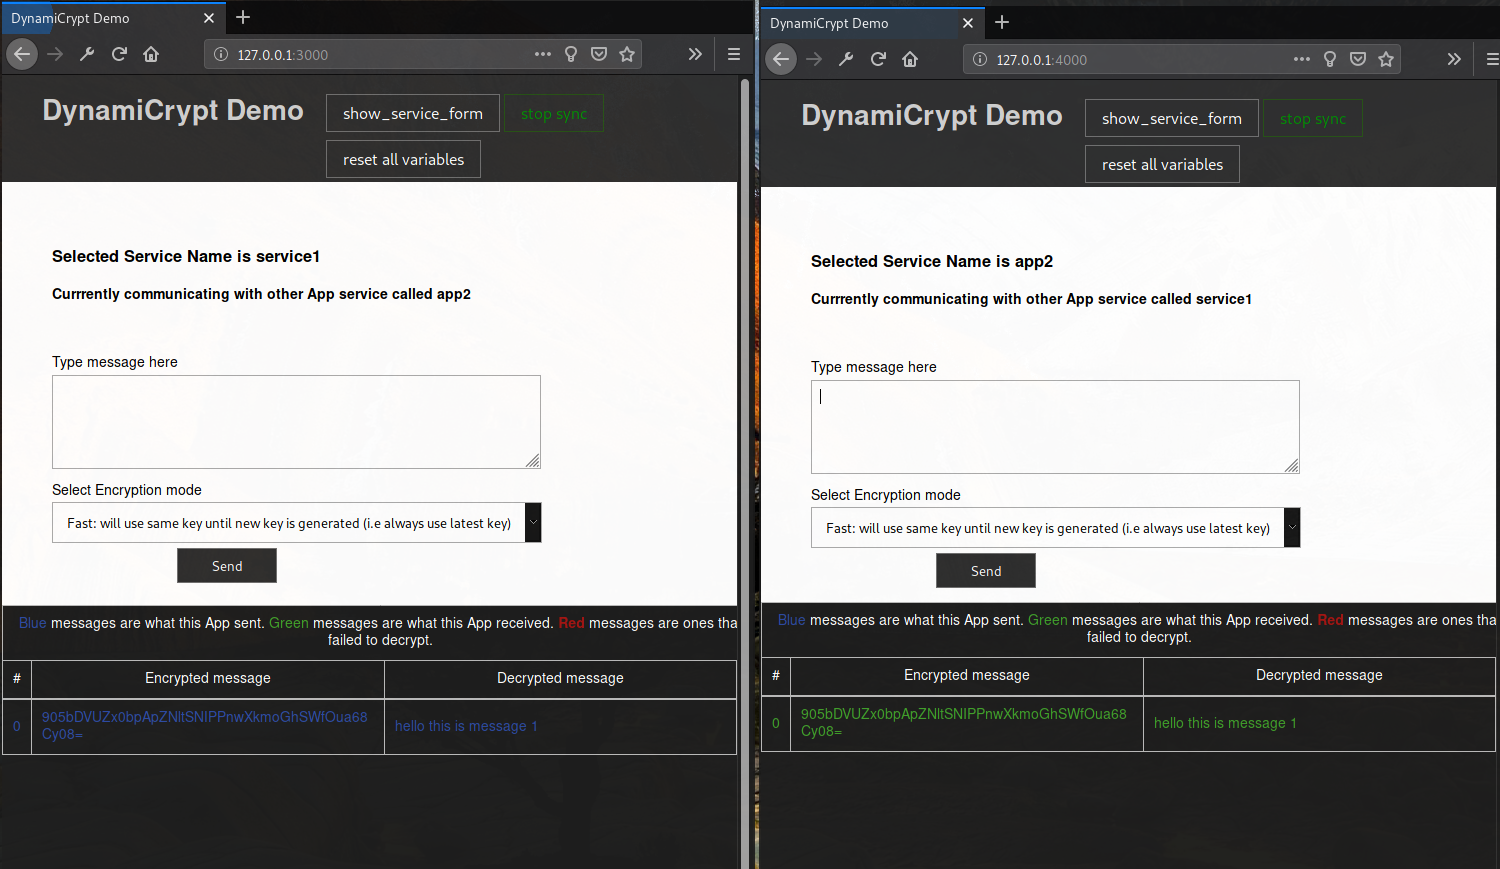
\includegraphics[width=1\textwidth]{Figures/b13.png}
  \caption[Encryption Node App view]{Encryption Node App view}
  \label{fig:b13}
\end{figure}
\FloatBarrier

Figure \ref{fig:b13} shows the two node Apps after a message "hello this is message 1" was sent using the text box interface of the left App. As you can see the right node App decrypted the text successfully.
I will use Wireshark once again to show the data sent between the Node Apps and the API.

\begin{figure}[!h]
  \centering
      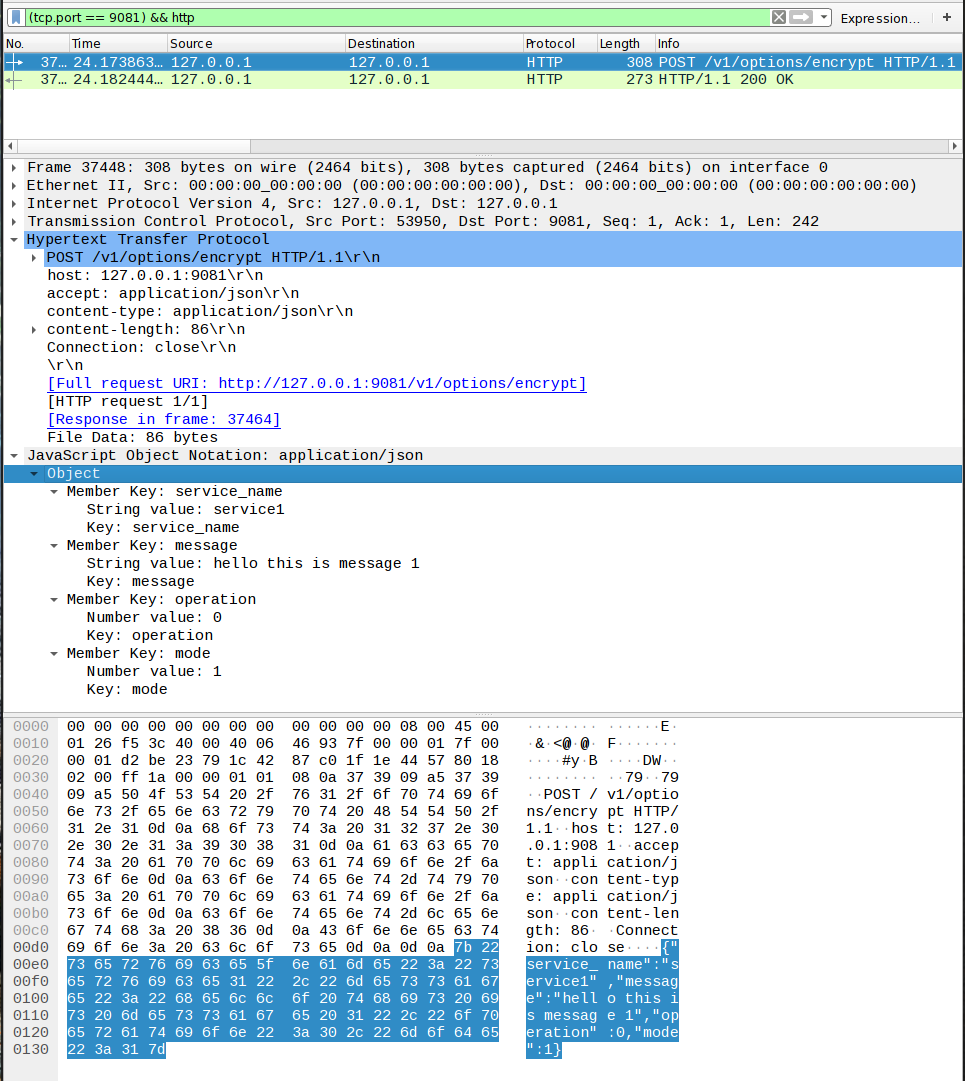
\includegraphics[width=1\textwidth]{Figures/b11.png}
  \caption[Node sends encryption message to the API ]{Node sends encryption message to the API}
  \label{fig:b11}
\end{figure}
\FloatBarrier
Figure \ref{fig:b11} shows the node app at port 3000 sending a post request to the encrypt route of the API.
The data it sends are as follows, service name so the API can identify which key store is appropriate for this service, message the plaintext that will be encrypted, operation this just means whether to encrypt or decrypt because the same route is used, in this case it is 0 but for decryption it would be 1. And finally the encryption mode, mode 1 was chosen in this case.

\begin{figure}[!h]
  \centering
      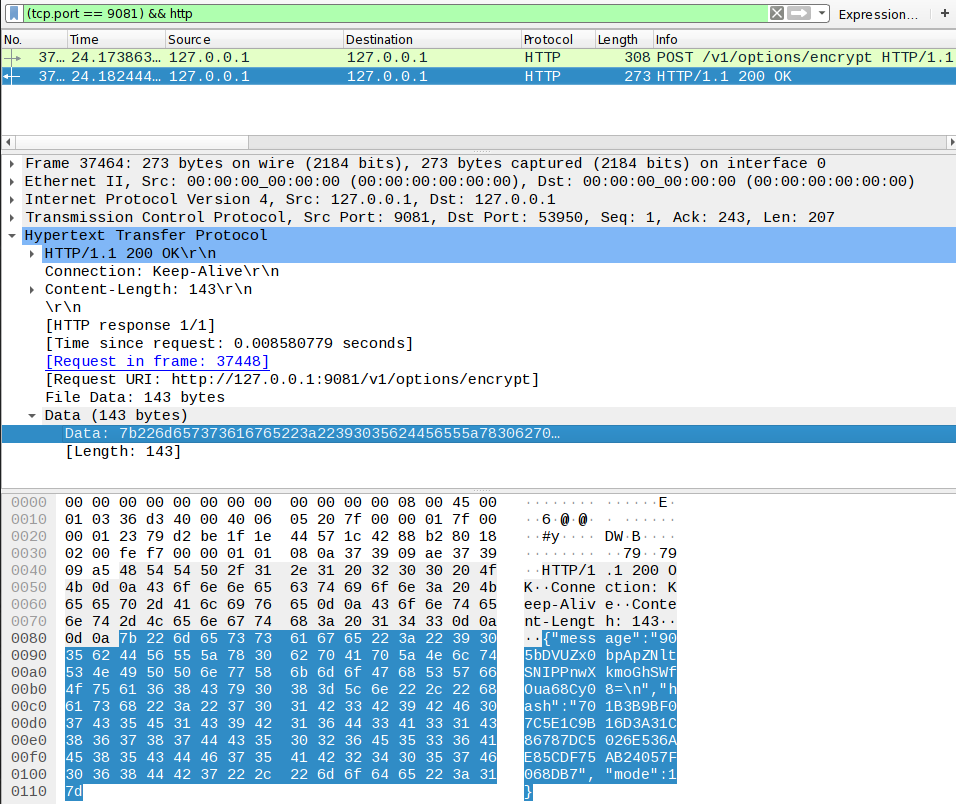
\includegraphics[width=1\textwidth]{Figures/b12.png}
  \caption[API responds with ciphertext and hash]{API responds with ciphertext and hash}
  \label{fig:b12}
\end{figure}
\FloatBarrier
Figure \ref{fig:b12} shows the response of the API, the API replies with the ciphertext as the message, followed by the hash of the plaintext and the mode to be used for decryption. This data will then be forwarded to the other node App by posting it to its decrypt route as seen in figure \ref{fig:b16}


\begin{figure}[!h]
  \centering
      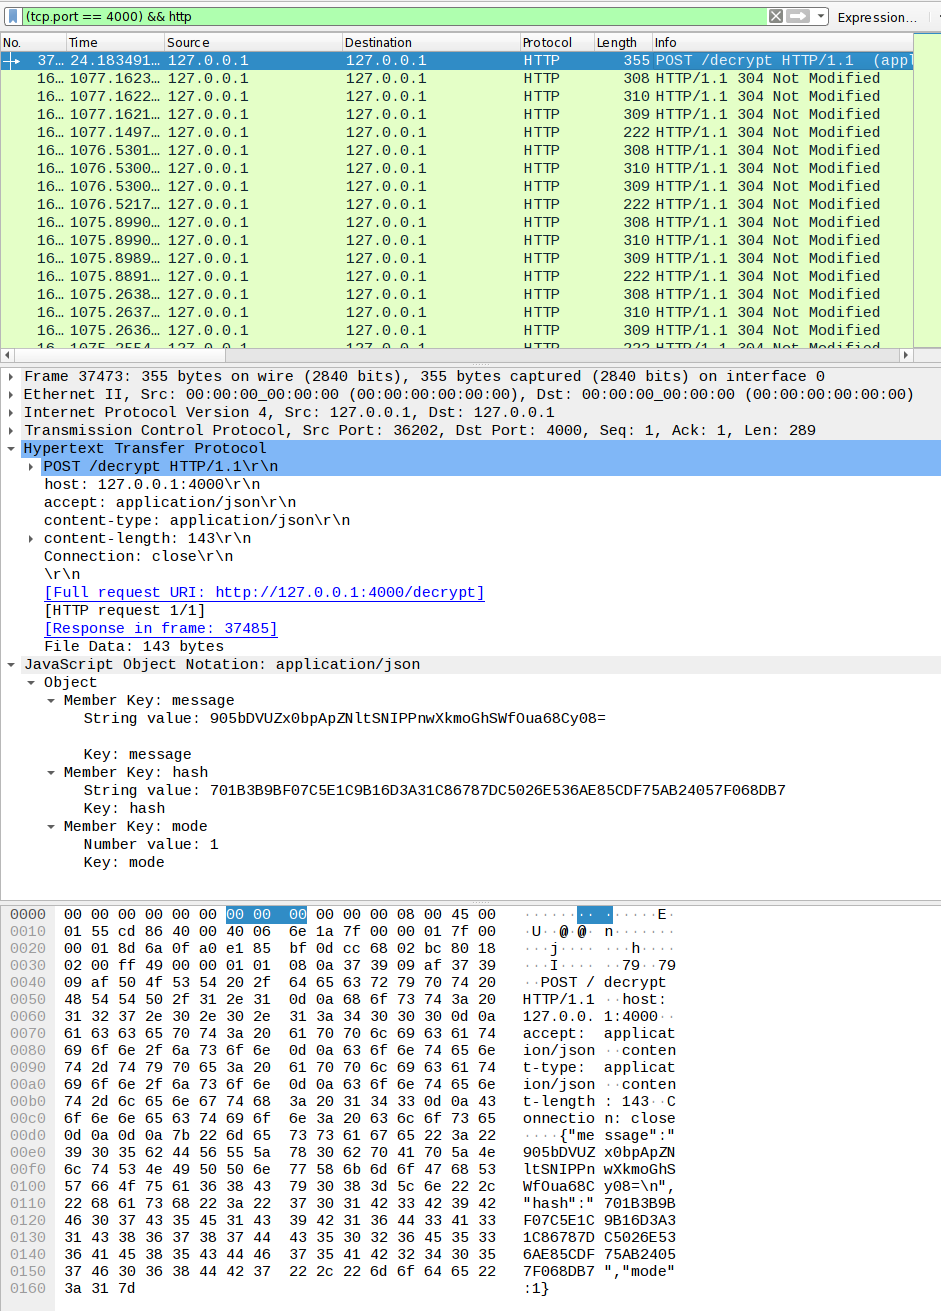
\includegraphics[width=1\textwidth]{Figures/b16.png}
  \caption[Node App at port 3000 sends ciphertext to Node App at port 4000 ]{Node App at port 3000 sends ciphertext to Node App at port 4000 }
  \label{fig:b16}
\end{figure}
\FloatBarrier


\begin{figure}[!h]
  \centering
      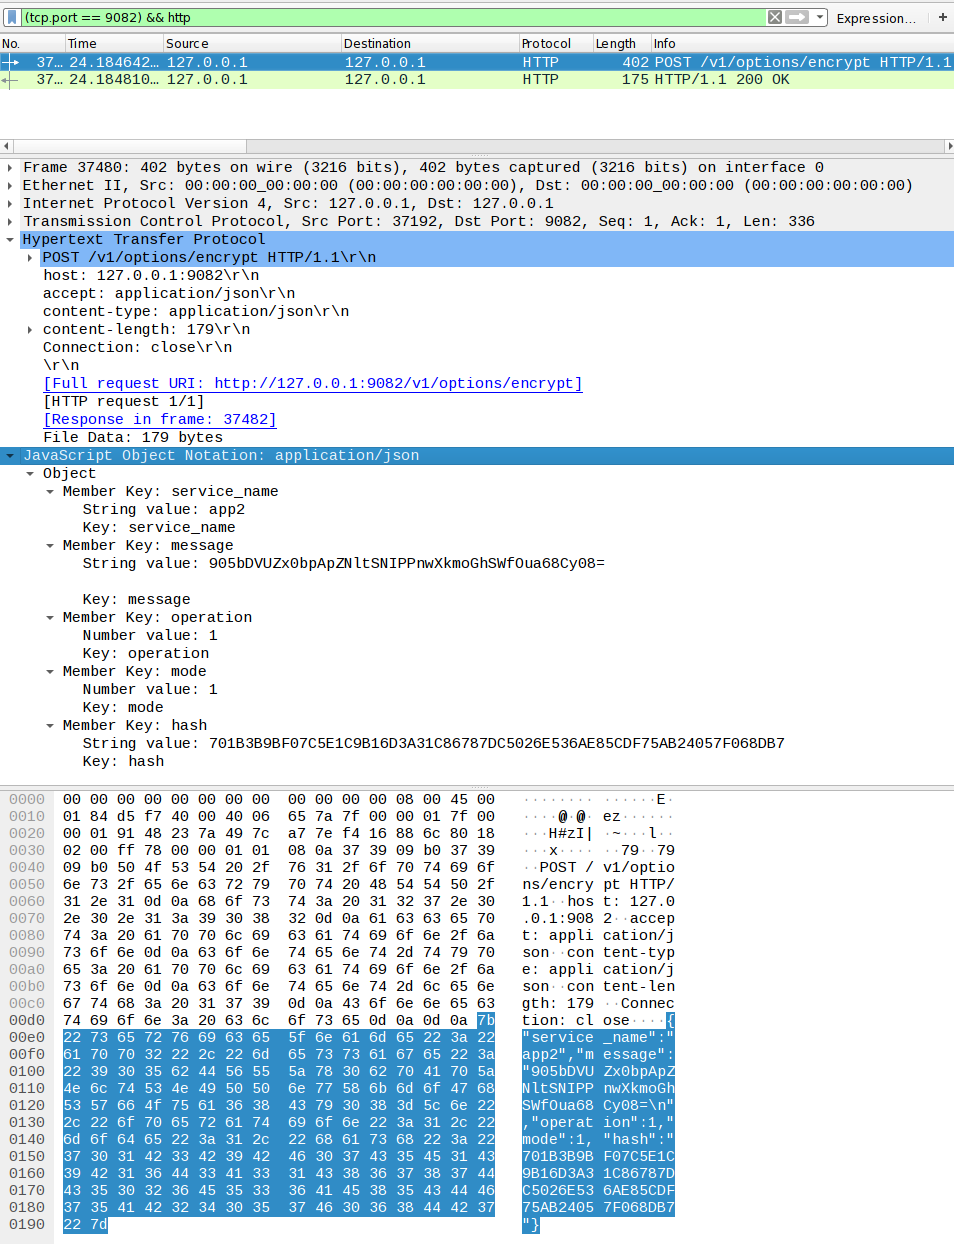
\includegraphics[width=1\textwidth]{Figures/b14.png}
  \caption[Node sends decryption message to the API ]{Node sends decryption message to the API }
  \label{fig:b14}
\end{figure}
\FloatBarrier

Now the node app on port 4000 needs to decrypt the ciphertext so it sends over its service name, ciphertext, operation is 1 this time for decryption, mode is 1 again and finally the hash of the plaintext forwarded from the other API to the API it is using on port 9082. This can all be seen in figure \ref{fig:b14}


\begin{figure}[!h]
  \centering
      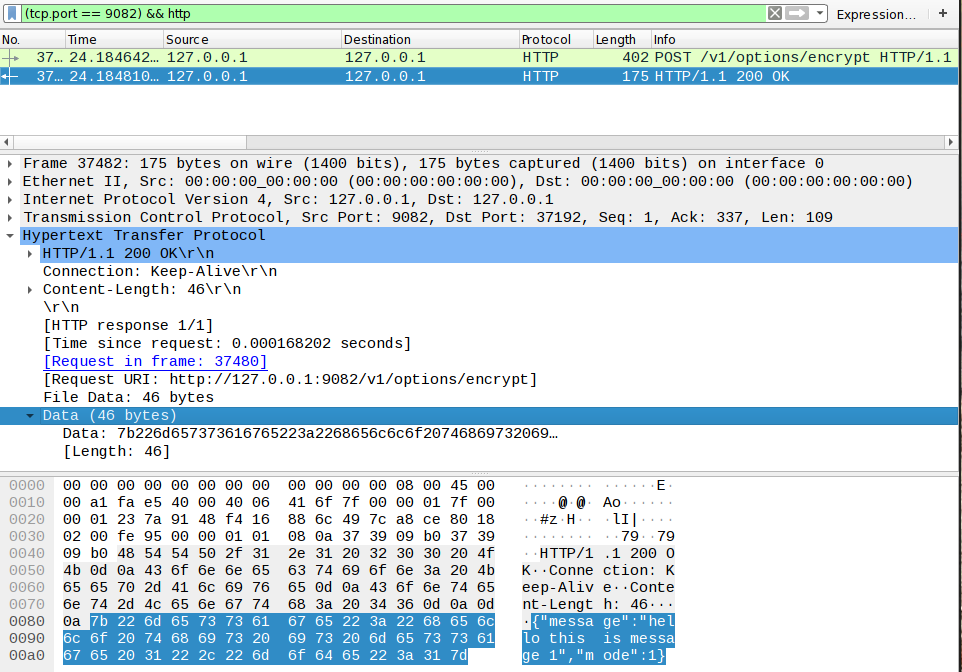
\includegraphics[width=1\textwidth]{Figures/b15.png}
  \caption[API responds with plaintext]{API responds with plaintext}
  \label{fig:b15}
\end{figure}
\FloatBarrier

Figure \ref{fig:b15} is a response from the API, the message was decrypted successfully and is simply sent back to the node app in plaintext the mode is also attached but this is not required for anything other than statistics. 


Next I would like to demonstrate the difference between the encryption modes using the node apps. Basically the point here is that if sending the same message i.e the same plaintext over and over in a non dynamic encryption environment the cipher text that will be produced will always be the same. 
You can see the following demonstration in video form which I mentioned before at this link https://www.youtube.com/watch?v=LsR4XsGrDCY&t=70s

Therefore since this project is all about dynamic encryption the ciphertext will be different every time if using the same plaintext. Note that it is guaranteed to be different every time if mode 2 is used since that will use a unique key for each message, mode 1 on the other hand is built for speed and therefore will use the latest available key therefore if frequent identical plaintexts are sent then there is a possibility that some of the ciphertexts will be the same. 

To test this properly a human would be too slow to type out the message each time so once again I will use a script which will basically submit the form on the browsers behalf. This python script is called send message.py and is once again located inside the GitHub repository.
The script looks like this.
\begin{lstlisting}
#!/usr/bin/env python3.7

import requests
import time

Service_address = "127.0.0.1"
Service_port = 3000

message = "hello -> using mode 1"
encrypt_mode = 1	# 1 for fast. i.e. encrypt using the latest key. 2 for secure only use 1 key once.

how_many_times = 10

url1 = "http://" + Service_address + ":" + str(Service_port) + "/encrypt"
data = {'message':message, 'encrypt_mode': encrypt_mode}

for i in range(0,how_many_times,1):
	print("sending")
	 
	r = requests.post(url = url1, data = data) 
	time.sleep(0.6)
\end{lstlisting}
As you can see this will send the message "hello -> using mode 1" to the encrypt route of the node app on port 3000 ( yes both the node app and the API have an encrypt route, only realised this might be confusing just now ).
This message will be sent 10 times and after each message is sent there will be a break for 0.6 seconds.
Firstly I will use encrypt mode 1.


\begin{figure}[!h]
  \centering
      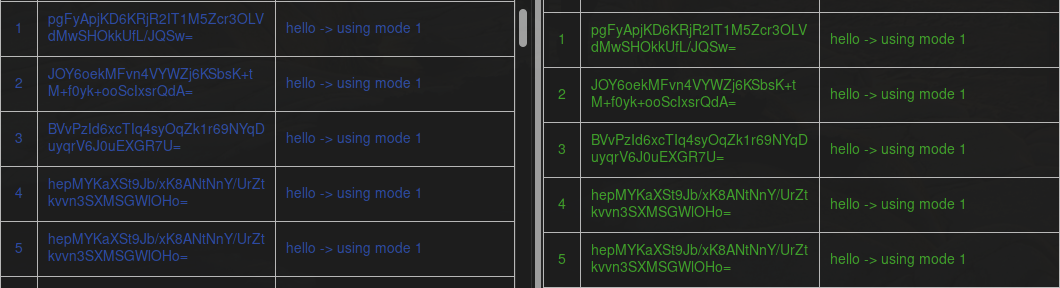
\includegraphics[width=1\textwidth]{Figures/b17.png}
  \caption[Encryption / Decryption mode 1 part 1]{Encryption / Decryption mode 1 part 1}
  \label{fig:b17}
\end{figure}
\FloatBarrier

\begin{figure}[!h]
  \centering
      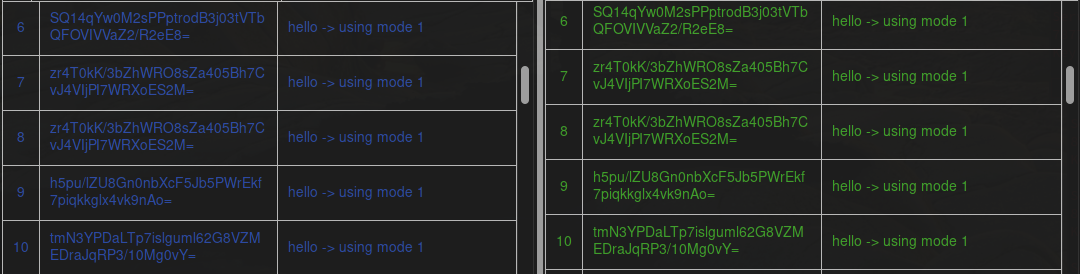
\includegraphics[width=1\textwidth]{Figures/b18.png}
  \caption[Encryption / Decryption mode 1 part 2]{Encryption / Decryption mode 1 part 2}
  \label{fig:b18}
\end{figure}
\FloatBarrier

Figures \ref{fig:b17} and \ref{fig:b18} show the output of the encryption and decryption table in the NodeJs apps after running the script. Here the plaintext is all the same and as you can see on the right node app they have decrypted successfully. The purpose of this test is to examine the cipher text and see which ones if any used the same key.
message 1 used a key unique to itself.
message 2 used a key unique to itself.
message 3 used a key unique to itself.

however message 4 and 5 have the same ciphertext therefore they have used the same key this is because by the time message 5 was encrypted no need key was generated yet and since this is mode 1 it just used the latest key available which happened to be the same one as message 4.

message 6 used a key unique to itself.

message 7 and 8 once again used the same key as each other.

message 9 used a key unique to itself.

message 10 used a key unique to itself.

Given that only two plaintexts were encrypted using the same key twice this is actually a very good result for mode 1. In my previous testing normally you would see three messages in a row encrypted with the same key. This time the keys were generated quicker than expected. How keys are generated will be covered in the sync-server section after this API section. 

Now we will have a look at using mode 2 for encryption to use mode 2 I simply modified two variables in the script.
\begin{lstlisting}
message = "hello -> using mode 2"
encrypt_mode = 2
\end{lstlisting}

\begin{figure}[!h]
  \centering
      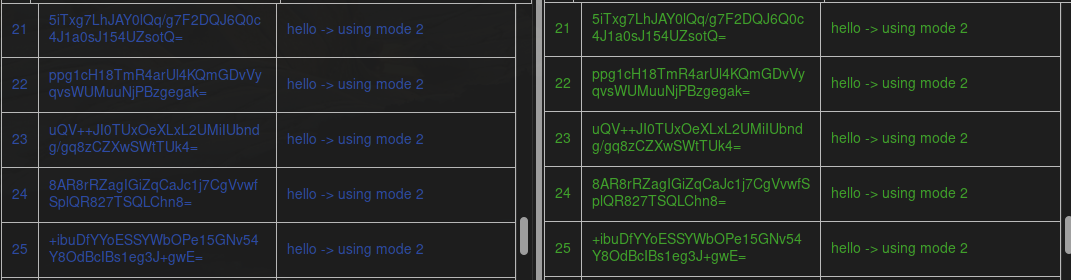
\includegraphics[width=1\textwidth]{Figures/b19.png}
  \caption[Encryption / Decryption mode 2 part 1]{Encryption / Decryption mode 2 part 1}
  \label{fig:b19}
\end{figure}
\FloatBarrier

\begin{figure}[!h]
  \centering
      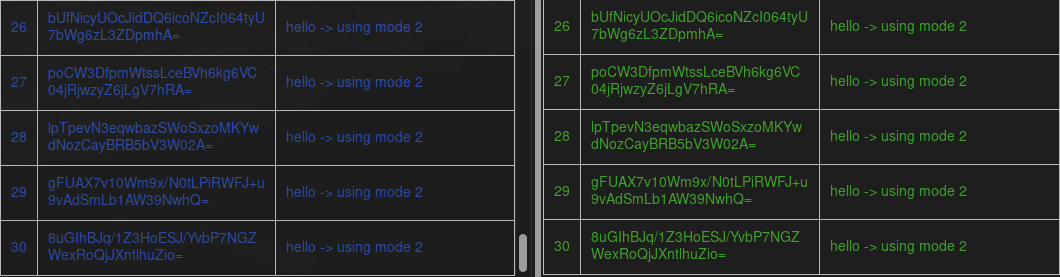
\includegraphics[width=1\textwidth]{Figures/b20.png}
  \caption[Encryption / Decryption mode 2 part 2]{Encryption / Decryption mode 2 part 2}
  \label{fig:b20}
\end{figure}
\FloatBarrier
Figures \ref{fig:b19} and \ref{fig:b20} show the output of the encryption and decryption table in the NodeJs apps after running the script with the modifications.
By looking at the ciphertexts part of the table of the Apps you can see that they are all different despite the same plaintext being used, therefore each message was encrypted using its own unique key and decrypted successfully as can be seen on the right app. 

This means that my algorithm works perfectly for both modes of operation.

As we can see both modes demonstrated dynamic cryptography. Mode 2 is in my opinion is more secure as each message no matter what is encrypted using a unique key. However there is a possibility that you will run out of suitable keys if sending loads of data frequently. If this happens you will just have to wait a little bit for new keys to be generated and encrypt again. 
Mode 1 therefore is perfect if you would like to send loads of data at regular intervals since there will be no issue with running out of keys, you will still reap the benefits of dynamic encryption since it takes around one second or so to generate new keys ( testing time of key generation will be seen later ). 

This will conclude the explanation and testing of aspects related to the API. If I were to explain everything related to the API it would take another 50 pages or so to go through everything therefore I selected the most impact full aspects of the API based on the outcomes of the project and left out most of the technical aspects. This section should have provided a good understanding of most of the more important operations of the API, it is recommended to browse through the GitHub repository for a full exposure of the API.

\section{Sync-server}
This section of the Document will cover the sync-server that is responsible for managing the Tree parity machines. As it was mentioned before the sync-server uses a custom peer to peer network where there are essentially two types of peers. One type is the one that waits for another peer to connect to it and the second type is the one that connects to the waiting peer. This is because there is no need to use a full fledged peer to peer network for the purposes required for DynamiCrypt there is no need for all the other features that come with a proper peer to peer network like peer discovery and such.

Since I used Boost Asio for the sync-server it is slightly different in the way the API was written since that used Pistache for networking. With boost asio a call back asynchronous architecture was used, Boost Asio also supports futures and promises however they were not covered deeply in the Book I used to learn Boost Asio. Nevertheless call backs are perfectly fine and efficient. 

The class that contains all of the interactions with sockets and directly with the network is the peer class. There is actually no such a thing as Sync-server code wise, I just refer to everything else that is not the API and not the Tree Parity Machine as Sync-server. This is because there are many peer objects stored in a vector which is global and there are functions for creating new peers, updating current and deleting unused peers inside definitions.cpp, which is not a class its just another source file from which some other class can call functions from if they included the appropriate header definitions.hpp.

As mentioned before there are two types of peers the only difference between these two is in the start function as seen here.
\begin{lstlisting}
void peer::start(std::string service_name, std::string partner_name){
	{ boost::recursive_mutex::scoped_lock lk(read_lock);
		peers.push_back( shared_from_this());
	}
	started_ = true;
	service_name_ = service_name;
	if(sock_using_ep){ // this makes the connection so write straight away
		//endpoint_(ip::address::from_string(ip_address_), ip_port_);
		endpoint_ = boost::make_shared<boost::asio::ip::tcp::endpoint>(boost::asio::ip::address::from_string(ip_address_), ip_port_);
		sock_.async_connect(*endpoint_, MEM_FN3(on_connect,_1,service_name,partner_name));
	} else { // this will listen to connection so read.
		do_read();
	}
}
\end{lstlisting}
As you can see the variable sock-using-ep determines which type of peer this is. This is set when creating a peer object and basically means is the socket that this peer will use be of type endpoint or not. If so then the address and port of another peer on the network will be loaded up and an asynchronous connection is made to the other peer.
\begin{lstlisting}
sock_.async_connect(*endpoint_, MEM_FN3(on_connect,_1,service_name,partner_name));
\end{lstlisting}
Because call backs are used a callback function must be provided which runs when the peer establishes a TCP connection with another peer. This call back function is on-connect, the service name and partner name are also passed in to be verified by the other peer ( more on this later ). 
If the peer is of type waiting then it simply waits for a peer to connect to it on the do-read function.
\begin{lstlisting}
void peer::do_read(){
	{ boost::recursive_mutex::scoped_lock lk(read_lock);
		async_read(sock_,  boost::asio::buffer(read_buffer_), MEM_FN2(read_complete,_1,_2), MEM_FN2(on_read,_1,_2));
	}
}
\end{lstlisting}
This read function performs an asynchronous read operation this time there are two call back functions read complete and on read, this is required because Boost asio doesn't know when all of the data is sent because you can configure it anyway you want. read complete basically scans the buffer for a newline character as that is what is set to determine the end of the TCP message and returns a boolean.
\begin{lstlisting}
size_t peer::read_complete(const boost::system::error_code & err, size_t bytes){
	if ( err) return 0;
	bool found = std::find(read_buffer_, read_buffer_ + bytes, '\n') < read_buffer_ + bytes;
	return found ? 0 : 1;
}
\end{lstlisting}
When this returns 1 Boost Asio then knows that the message has been fully read and calls the on read function which can then access the read buffer and perform calculations on the message.

\begin{figure}[!h]
	\centering
	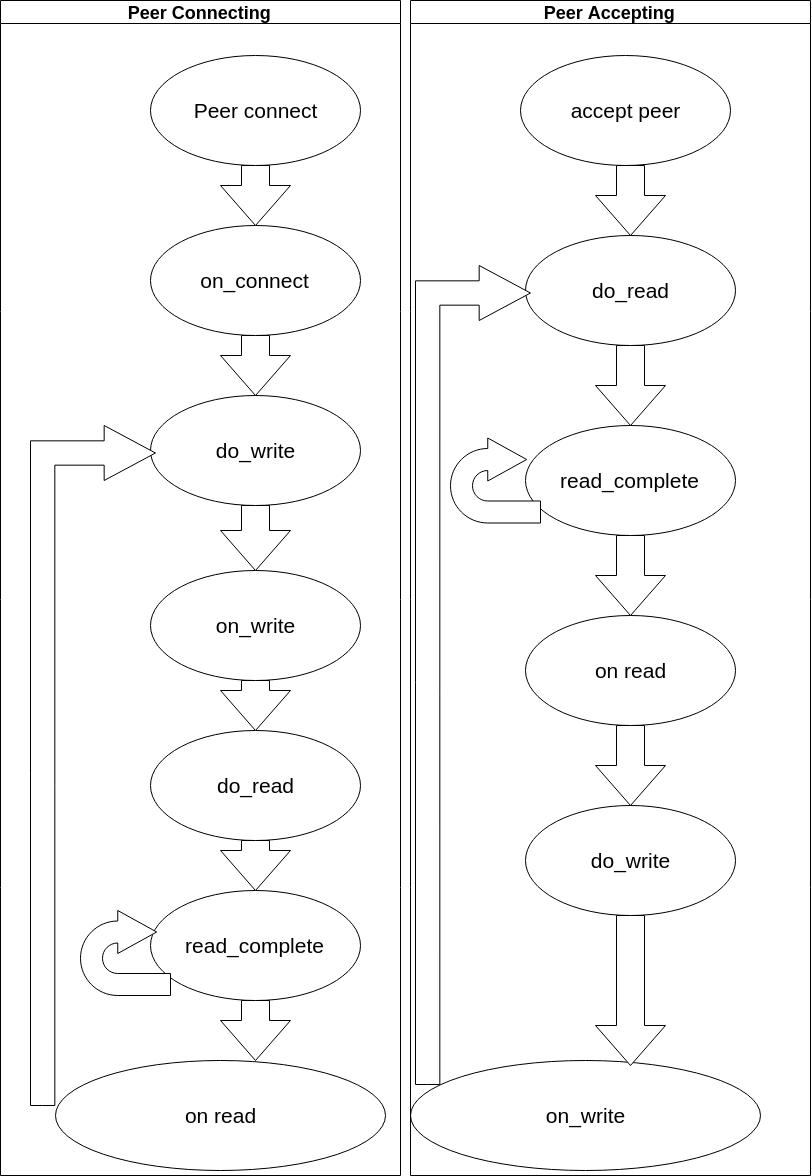
\includegraphics[width=1\textwidth]{Figures/sync_code_flow-modded.png}
	\caption[Asynchronous flow diagram of peer]{Asynchronous flow diagram of peer}
	\label{fig:s1}
\end{figure}
\FloatBarrier

Before continuing with the rest of the operations a quick overview of the asynchronous code flow is presented in figure \ref{fig:s1}. The two boxes represent the two different peers and the order of the asynchronous operations that they follow. 
The connecting peer after connecting to a reading peer prepares a packet and and calls the do write operation. After the do write operation finishes writing all of the data to the socket on write is called which then calls do read, then read complete gets called multiple times until a newline character is detected, then on read is called and there are other functions called from on read that call do write and the cycle continues.

The accepting peer as referred in the diagram is the waiting peer. It is important for the connecting peer and waiting peer to not read or write to the socket at the same time, so you will notice that every time the connecting peer is writing the accepting peer is reading and visa-versa.  
The waiting peer starts of its cycle by reading since there is no data on the socket while there is no peer that is about to connect it simply does nothing. Boost Asio in the background does check periodically for any data in the socket but this behaviour is hidden from the developer. After a peer connects to the waiting peer it immediately starts checking if the message was fully sent by repeatedly calling read complete when a new byte arrives. When all the data is received on read is called which creates a new message and calls do write when the message is fully written on write is called which once again calls do read and the cycle once again continues.

Currently there are four types of messages or at least four different categories of messages. Messages are constructed in the following fashion message-type + tab character + data + tab character + data + ...... + new line character.

Messages of message-type 1 are used for sending synchronisation data used to synchronise tree parity machines.

Messages of message-type 2 are used for when the peer initially connects to another peer this is the first message in the conversation.

Messages of message-type 3 are essentially a reply to message-type 1 with more information needed to setup the tree parity machines.

Messages of message-type 4 are for resetting tree parity machines if a key is found, or if the tree parity machines reached the maximum iteration count

Bellow is a snippet of all the different types of messages and the function from which they are called from.

\begin{lstlisting}
Note the << operator in C++ just adds data to a buffer so ss << "1" << variable << "string" would be the same as ss = "1" + variable + "string" in something like python for example.


// called from std::string TpmNetworkHandler::sync_tpm_message_one(int tpm_id)
ss << "1\t" << tpm_id << "\t" << tpm_networks_[index].id() << "\t" << tpm_networks_[index].iteration() << "\t" << random_input_vector << "\t" << tpm_result << "\t" << 1 << "\n";
  
  
// called from std::string TpmNetworkHandler::sync_tpm_message_one_advanced(int tpm_id, std::vector<std::string> & parsed_msg)
ss << "1\t" << tpm_id << "\t" << tpm_networks_[index].id() << "\t" << tpm_networks_[index].iteration() <<  "\t" << random_input_vector << "\t" << tpm_result << "\t" << message_type_to_process  << "\t" << tell_machine_to_update<< "\t" << old_input_vector << "\t" << key_hash << "\t" << random_input_for_key << "\n";


// called from void peer::on_connect(const error_code & err, std::string service_name, std::string partner_name)
ss << "2\t" << id << "\t" << tpm_handler.get_iteration(id) << "\t" << service_name << "\t" << partner_name << "\n";

// called from void peer::on_init(std::vector<std::string> & parsed_msg)
ss << "3\t" << id << "\t" << tpm_handler.get_iteration(id) << "\t" << tpm_handler.get_partner(id) << "\n";


// called from void peer::on_sync(std::vector<std::string> & parsed_msg) and void peer::on_linking(std::vector<std::string> & parsed_msg) also uses the same parameters
ss << "4\t" << tpm_id << "\t" << tpm_handler.get_iteration(tpm_id) << "\t" << 0 << "\t" << 0 << "\n";


// called from std::string TpmNetworkHandler::sync_tpm_message_one_advanced(int tpm_id, std::vector<std::string> & parsed_msg)
ss << "4\t" << tpm_id << "\t" << tpm_networks_[index].iteration() << "\t" << 0 << "\t" << 1 << "\n";
\end{lstlisting}

The on read function is the first function to receive the complete message. 
\begin{lstlisting}
void peer::on_read(const error_code & err, size_t bytes){
	if ( err) stop();
	if ( !started() ) return;
	// process the msg
	std::string msg(read_buffer_, bytes);
	msg.pop_back();
	std::vector<std::string> parsed_msg; 
	boost::split(parsed_msg, msg, [](char c){return c == '\t';});
	// partner id \t partners iteration
	if(std::stoi(parsed_msg.at(0)) == 1){ // message type 1;
		if(PRINT_SYNC_MESSAGES){
			std::cout << "message type 1 received" << "with partner id of " << parsed_msg.at(1) << " and iteration " << parsed_msg.at(3) <<  std::endl;
		}
		on_sync(parsed_msg);
	} 
	// init tree parity machines
	else if(std::stoi(parsed_msg.at(0)) == 2){
		std::cout << "message type 2 received" << "with partner id of " << parsed_msg.at(1) << " and iteration " << parsed_msg.at(2) <<  std::endl;
		on_init(parsed_msg);
	}
	// link inited tree parity machines
	else if(std::stoi(parsed_msg.at(0)) == 3){
		std::cout << "message type 3 received" << "with partner id of " << parsed_msg.at(1) << " and iteration " << parsed_msg.at(2) << " and self id of " <<  parsed_msg.at(3) << std::endl;
		on_linking(parsed_msg);
	}
	// reset tree parity machines or stop
	else if(std::stoi(parsed_msg.at(0)) == 4){
		std::cout << "message type 4 received" << "with partner id of " << parsed_msg.at(1) << " and iteration " << parsed_msg.at(2) << " and stop tpm " <<  parsed_msg.at(3) << std::endl;
		on_reset(parsed_msg);
	}
	else std::cerr << "invalid msg " << msg << std::endl;
}
\end{lstlisting}
As you can see the on read function is rather small as all it does is split the message at the tabbed character into a vector using a split function from boosts library. 
Then the vector is sent to the appropriate function for handling the appropriate message. 
From the code above you can see that all messages with 1 at the beginning go to the sync function, messages with 2 go to the init function, messages with 3 go to the linking function, messages with 4 go to the reset function and all other messages are ignored since they shouldn't be there in the first place.

\textbf{Sync-server execution walk through}

For this part of the thesis a real life example of how peers communicate with each other will take place.
To set this up for easier explanation the PRINT SYNC MESSAGES will be turned on and all of the output will be redirected into a file as seen in figure \ref{fig:sync1}.

\begin{figure}[!h]
	\centering
	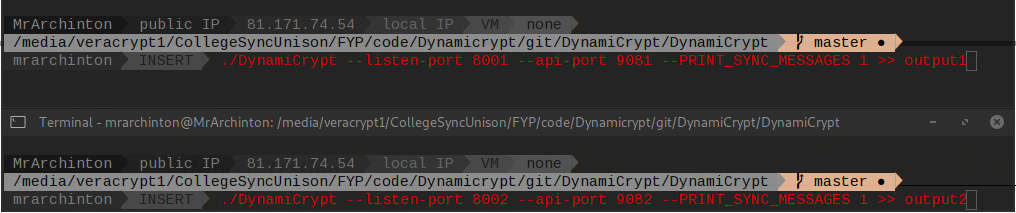
\includegraphics[width=1\textwidth]{Figures/sync1.png}
	\caption[DynamiCrypt execution arguments]{DynamiCrypt execution arguments}
	\label{fig:sync1}
\end{figure}
\FloatBarrier

The next steps are to connect two NodeJs apps as described in the API section and start up Wireshark before clicking the start sync button in one of the NodeJs apps.
For this setup the peer on the DynamiCrypt app on port 8001 will connect to the peer on DynamiCrypt app with port 8002. Since the first App is using a connecting type peer, that peer will choose a random port available so in order to filter out the extra traffic we will apply a filter for port 8002 since that is where the listening/waiting peer will be listening on. 
\begin{lstlisting}
(tcp.port == 8002) && (tcp.flags.push == 1)
\end{lstlisting}
The second filter simply gets rid of all other TCP traffic and keeps the data that is specifically generated by the peer.
When the connecting peer connects to the waiting peer it goes to the on connect function to generate the first message.
\begin{lstlisting}
void peer::on_connect(const error_code & err, std::string service_name, std::string partner_name){
			for(int b=0; b< MAX_TPMS_PER_PEER; b++){
				int id = tpm_handler.create_new_tpm(service_name, partner_name);
				
				if ( !err){      
					std::stringstream ss;                                               // send self service name
					ss << "2\t" << id << "\t" << tpm_handler.get_iteration(id) << "\t" << service_name << "\t" << partner_name << "\n";
					std::cout << "on_connect: " << ss.str() << std::endl;
					do_write(ss.str());
				}
				else{
					std::cout << "Error on_connect:" << err.message() << std::endl;
					api_service_data_handler.remove_service(service_name);
					stop();
				}
			}
	}
\end{lstlisting}
Before sending data tree parity machines are created to be used for synchronisation, in this case only one tree parity machine is created. The tpm handler object is using the TpmNetworkHandler class has a vector of SingleTpmNetworkHandler objects. The SingleTpmNetworkHandler class is just a wrapper for the actual tree parity machine object but with extra functions for networking and referencing purposes. 
After creating a tree parity machine with id 702 as can be seen from the output1 file the first message is constructed it is of type message 2.
\begin{lstlisting}
created new tpm with id 702
on_connect: 2	702	0	service1	app2
\end{lstlisting}
What this means is that for the NodeJs app with the service name service1 the tree parity machine with the id 702 will be used, the partner service name is also sent for linking reasons. 
This string is then sent over the network to the other peer as can be seen in Wireshark figure \ref{fig:sync3}. Note Wireshark doesn't render tabbed characters so in the data section it just looks like spaces where there is actually the tabbed character.
\begin{figure}[!h]
	\centering
	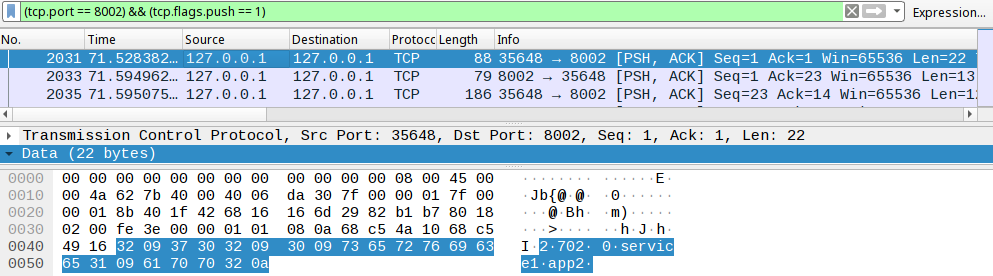
\includegraphics[width=1\textwidth]{Figures/sync3.png}
	\caption[peer message type 2]{peer message type 2}
	\label{fig:sync3}
\end{figure}
\FloatBarrier

This is then received by the other peer as seen in the output2 file.
\begin{lstlisting}
message type 2 receivedwith partner id of 702 and iteration 0
\end{lstlisting}
All messages of type two are handed of to the on init function
\begin{lstlisting}
void peer::on_init(std::vector<std::string> & parsed_msg){
		std::cout << "on_init service_name is " << parsed_msg.at(4);
		std::cout << " partners service name is " << parsed_msg.at(3) << std::endl;
		
		service_name_ = parsed_msg.at(4); //needed for when type of peer is accepting
		int id = tpm_handler.create_new_tpm(parsed_msg.at(4),parsed_msg.at(3));
		tpm_handler.set_partner(id, std::stoi(parsed_msg.at(1)));
		
		std::stringstream ss;
		ss << "3\t" << id << "\t" << tpm_handler.get_iteration(id) << "\t" << tpm_handler.get_partner(id) << "\n";
		std::cout << " on_init: " << ss.str() << std::endl;
		do_write(ss.str());
}
\end{lstlisting}
Here is the standard output for this function.
\begin{lstlisting}
on_init service_name is app2 partners service name is service1
Read random value: 17697991126802347472
random number: 17697991126802347472
writing to file
created new tpm with id 3141
on_init: 3	3141	0	702
\end{lstlisting}
This peer also creates a new TPM for the other NodeJs app with the service name app2. The random number seen here in the output is just the number that's used for the seed, read from /dev/urandom when generating weights for the tree parity machines. The tree parity machine that's created for app2 has the id of 3141, when creating the tree parity machine the service1 tree parity machines id was passed this is so that a partner set of tree parity machines only communicate with themselves and no other tree parity machine in the vector. 

This function then creates a message of type 3 with its tree parity machine id and the id of the partner tree parity machine and sends it to the other peer as can be seen in the Wireshark in figure \ref{fig:sync4}.

\begin{figure}[!h]
	\centering
	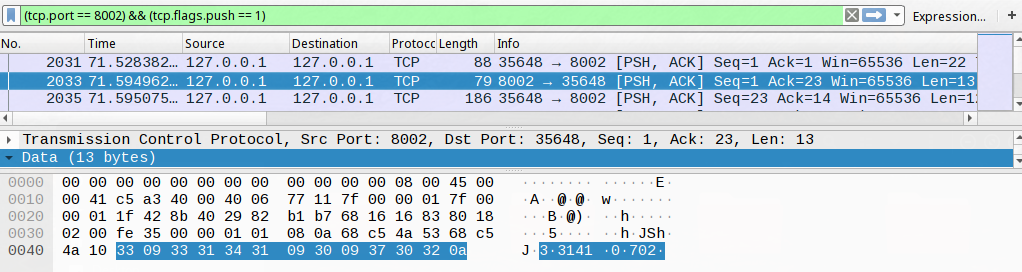
\includegraphics[width=1\textwidth]{Figures/sync4.png}
	\caption[peer message type 3]{peer message type 4}
	\label{fig:sync4}
\end{figure}
\FloatBarrier

When the peer receives this message it is forwarded to the on linking function.
\begin{lstlisting}
//from file output1 
message type 3 receivedwith partner id of 3141 and iteration 0 and self id of 702
\end{lstlisting}
\begin{lstlisting}
void peer::on_linking(std::vector<std::string> & parsed_msg){
		bool tpm_found = false;
		bool tpm_reset = false;
		int tpm_index = tpm_handler.find_tpm(std::stoi(parsed_msg.at(3)), false);
		int tpm_id = -1;
		if(tpm_index != -1){
			tpm_found = true;
			tpm_id = tpm_handler.getid(tpm_index);
			if(!tpm_handler.increase_iteration(tpm_id)){
				//tpm_handler.reset_tpm(tpm_index);
				tpm_found = true;	
			}
			tpm_handler.set_partner(tpm_id, std::stoi(parsed_msg.at(1)));
		}     

		if(tpm_found){
			std::stringstream ss;
			if(tpm_reset){                                                                     // 1 = stop 
				ss << "4\t" << tpm_id << "\t" << tpm_handler.get_iteration(tpm_id) << "\t" << 0 << "\t" << 0 << "\n";
			}else{
				ss << tpm_handler.sync_tpm_message_one(tpm_id);
			}
			std::cout << "on_linking: " << ss.str() << std::endl;
			do_write(ss.str());
		}
		else{ // something is not right
			
			std::cout << "on_linking no tpm found" << std::endl;
			
		}
} 
\end{lstlisting}
Firstly this function finds the appropriate tree parity machine based on its id. Then increases the synchronisation iteration count since the first sync message will be sent at the end of this function. Then updates this tree parity machine with the id of the partner tree parity machine id in this case that would be 3141. 

Then a call is made to the tpm handler object to create the first sync message.
\begin{lstlisting}
std::string TpmNetworkHandler::sync_tpm_message_one(int tpm_id){
	std::stringstream ss;
	int index = find_tpm(tpm_id, false);
	
	std::string random_input_vector = tpm_networks_[index].create_random_input_vector();
	int tpm_result = tpm_networks_[index].compute_tpm_result();
	
	// id, itteration, randomVector, resultOfVector
	ss << "1\t" << tpm_id << "\t" << tpm_networks_[index].id() << "\t" << tpm_networks_[index].iteration() << "\t" << random_input_vector << "\t" << tpm_result << "\t" << 1 << "\n";
	
	if(PRINT_SYNC_MESSAGES){
		std::cout << "sync_tpm_message_one end" << std::endl;
	}
	return ss.str();
	
	// sends random vector and result to said random vector but doesn't update weights.
}   
\end{lstlisting}
This function once again finds the appropriate tree parity machine by its id. Then creates a random input vector which is what the tree parity machines will use to synchronise. The tree parity machine then updates its neurons with this vector and calculates the output neuron which is either -1 or 1. 
Then the message is constructed with the tree parity machines id, sync iteration, the random input vector is also sent to be used by the other tree parity machine, the output of the tree parity machine calculation and the sync iteration. This message is then sent over the network as seen in figure \ref{fig:sync5}.
\begin{lstlisting}
// from file output1
sync_tpm_message_one end
on_linking: 1	702	702	1	-1111-1-1-111-111-1-1111111-1-11-11-11-111111-111-11-111-11-1-1-11-11111111-11-11-1-1-1-11-11-1-1-1-111	1	1
\end{lstlisting}

\begin{figure}[!h]
	\centering
	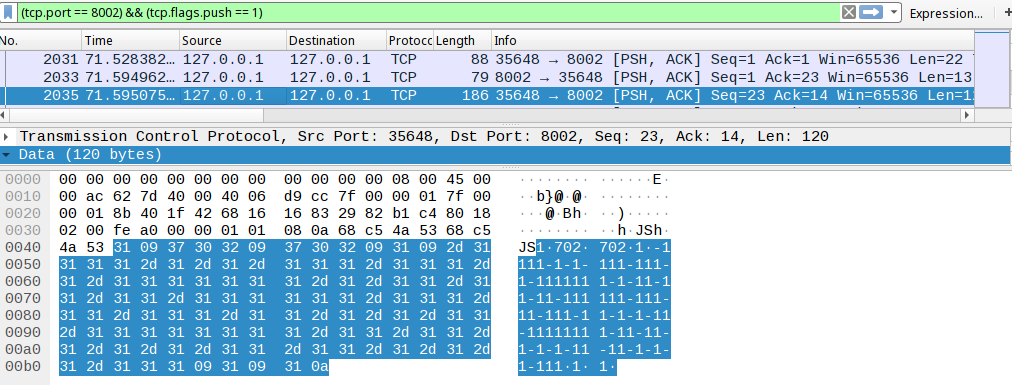
\includegraphics[width=1\textwidth]{Figures/sync5.png}
	\caption[peer message type 1]{peer message type 1}
	\label{fig:sync5}
\end{figure}
\FloatBarrier

\begin{lstlisting}
// from file output2
message type 1 receivedwith partner id of 702 and iteration 1
\end{lstlisting}

This time the on sync method is called since the message type is 1.
\begin{lstlisting}
void peer::on_sync(std::vector<std::string> & parsed_msg){
		bool tpm_found = false;
		bool tpm_reset = false;
		int tpm_index = tpm_handler.find_tpm(std::stoi(parsed_msg.at(1)), true);
		int tpm_id = -1;
		if(tpm_index != -1){
			tpm_found = true;
			tpm_id = tpm_handler.getid(tpm_index);
			
			if(!tpm_handler.increase_iteration(tpm_id)){
				//tpm_handler.reset_tpm(tpm_index);
				tpm_reset = true;
			}
		}
		
		if(tpm_found){
			std::stringstream ss;
			if(tpm_reset){                                                                     // 1 = stop 
				ss << "4\t" << tpm_id << "\t" << tpm_handler.get_iteration(tpm_id) << "\t" << 0 << "\t" << 0 << "\n";
			}else{
				ss << tpm_handler.sync_tpm_message_one_advanced(tpm_id, parsed_msg);
			}
			if(PRINT_SYNC_MESSAGES){
				std::cout << "on_sync: key_couter=" << tpm_handler.increase_key_counter(tpm_index) << std::endl;
			}else{
				tpm_handler.increase_key_counter(tpm_index);
			}
			do_write(ss.str());
		} else{ // must be new machine? but shouldnt be	
			std::cout << "on_sync no tpm found" << std::endl;
		}
}
\end{lstlisting}
This simply checks if the tree parity machine exists and checks if it needs to be reset if the iteration count is too high. Then to generate the next message the sync message one advanced is called from the tpm handler object. There are a few different functions for handling sync messages this is because the goal is to send as little messages over the network as possible so the functions do as much work as possible as you will see next.
The
\begin{lstlisting}
std::string TpmNetworkHandler::sync_tpm_message_one_advanced(int tpm_id, std::vector<std::string> & parsed_msg){
\end{lstlisting}
function is very long so only snippets of it will be produced. It supports two types of sync messages internally this is defined by the 7th element in the message this time we will be dealing with type 1.
\begin{lstlisting}
if(processing_message_type_now == 1){ // dont update ur weights straight away
	std::string random_vector_received = parsed_msg.at(4);
	old_input_vector = random_vector_received;
	int result_received = std::stoi(parsed_msg.at(5));
	tpm_networks_[index].set_random_input_vector_from_string(random_vector_received);
	int tpm_result_old = tpm_networks_[index].compute_tpm_result();
	
	if(tpm_result_old == result_received){
		tpm_networks_[index].update_weight();
		tell_machine_to_update = 1;
	}        
	
	random_input_vector = tpm_networks_[index].create_random_input_vector();
	tpm_result = tpm_networks_[index].compute_tpm_result();
	
	if(PRINT_SYNC_MESSAGES){
		std::cout << "sync_tpm_message_one_advanced-1 before getKey" << std::endl;
	}
	message_type_to_process = 2;
	//key = tpm_networks_[index].get_key();
	if(PRINT_SYNC_MESSAGES){
		std::cout << "tpm key gotten ok"<< std::endl;
	}
	random_input_for_key = gen_random_input_for_key(50);
	if(PRINT_SYNC_MESSAGES){
		std::cout << "random_input_gotten_ok"<< std::endl;
	}
	key_hash = tpm_networks_[index].calc_test(random_input_for_key);
	if(PRINT_SYNC_MESSAGES){
		std::cout << "key_hash_gotten_ok"<< std::endl;
		std::cout << "sync_tpm_message_one_advanced-1 end" << std::endl;
	}
	//std::cout << "\n\nok\n"; 
} 
\end{lstlisting}
This sets up the random vector received to be used for calculating the neurons. Then the output is calculated based on this vector. If the output of both tree parity machines match the weights will be updated. In this case the output of the tree parity machines are not the same so the weights are not updated.  
Then a new random input vector is created and the calculation for the output is performed. 

Then the  sync message type to handle by the other tpm is set to 2 since now there will be hashes involved.

Next a random input is generated this will be sent to the other tree parity machine along side a hash to check the key. 

Then a hash is calculated using the weights of the tree parity machine and the random input just mentioned.  
\begin{lstlisting}
std::string SingleTpmNetworkHandler::calc_test(std::string randomInput){
	std::string hashed_key = SHA256(get_key());
	std::string hashed_input = SHA256(randomInput);
	
	std::stringstream ss;
	for(int i=0; i < hashed_key.length(); i++){
		ss << hashed_key.at(i) << hashed_input.at(hashed_input.length() -i -1);
	}
	
	return SHA256(ss.str());
}
\end{lstlisting}
This function simply gets the hash of the key which is generated by the weights adds that to the random input hashed and then hashes the result of all of this once again to be safely sent across the network. Hashing different bits of data 3 times might be a bit over kill just for a simple test to see if the weights match but it is better to be safe than sorry.

Then finally all of this information is sent to the other peer.
\begin{lstlisting}
    if(PRINT_SYNC_MESSAGES){
std::cout << "\niteration " << tpm_networks_[index].iteration() << "message type: " << message_type_to_process << "tell_machine_to_update " << tell_machine_to_update << "\nkey_hashed: " << key_hash << "\nold: " << old_input_vector << "\nnew:" << random_input_vector << "\n\n";  
}

// mostly compatible with sync_tpm_message_one message.
ss << "1\t" << tpm_id << "\t" << tpm_networks_[index].id() << "\t" << tpm_networks_[index].iteration() <<  "\t" << random_input_vector << "\t" << tpm_result << "\t" << message_type_to_process  << "\t" << tell_machine_to_update<< "\t" << old_input_vector << "\t" << key_hash << "\t" << random_input_for_key << "\n";

return ss.str();
\end{lstlisting}
Here is the same output but with actual values as sent over the network and captured by Wireshark \ref{fig:sync6}.
\begin{figure}[!h]
	\centering
	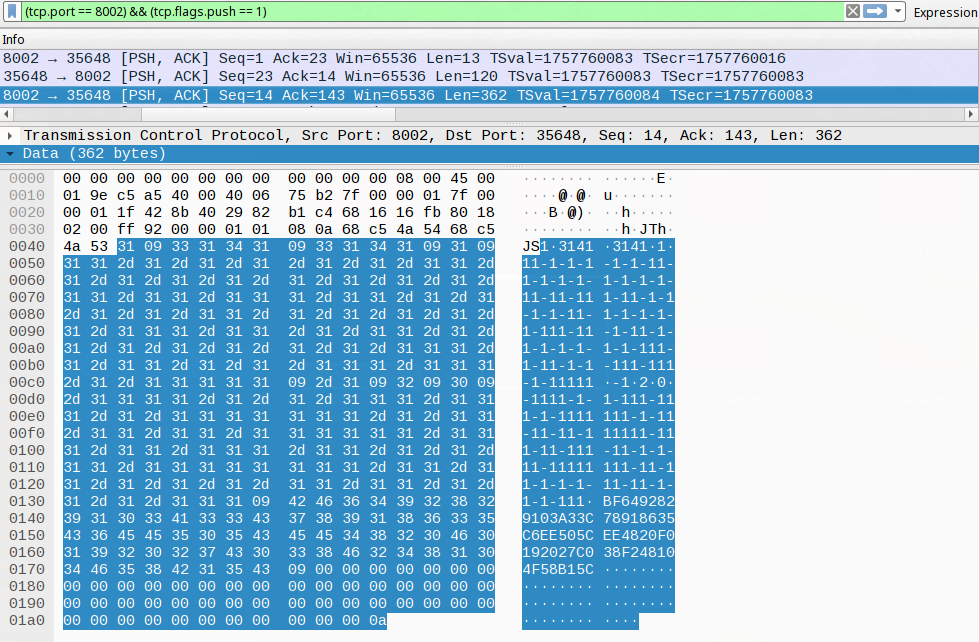
\includegraphics[width=1\textwidth]{Figures/sync6.png}
	\caption[peer message type 1 advanced]{peer message type 1 advanced}
	\label{fig:sync6}
\end{figure}
\FloatBarrier

When this message arrives at the peer outputting to file output1 it goes in to the same function as last time but into processing message type 2 this time.
\begin{lstlisting}
else if(processing_message_type_now == 2) {
	
	tell_machine_to_update = std::stoi(parsed_msg.at(7));
	//std::cout << "\n\nokkkk\n"; 
	if(tell_machine_to_update == 1){
		old_input_vector = parsed_msg.at(8);
		tpm_networks_[index].set_random_input_vector_from_string(old_input_vector);
		if(PRINT_SYNC_MESSAGES){
			std::cout << "\nupdating machine with this vector \n" << old_input_vector << "\n";
		}
		tpm_networks_[index].update_weight();
		
		std::string other_key = parsed_msg.at(9);
		//key = tpm_networks_[index].get_key();
		
		random_input_for_key = parsed_msg.at(10);
		key_hash = parsed_msg.at(9);
		
		std::string key_hash_this = tpm_networks_[index].calc_test(random_input_for_key);
		
		
		
		if (!key_hash.compare(key_hash_this)) {
			// keys are the same
			if(PRINT_SYNC_MESSAGES){
				std::cout << "found same key hash : " << key_hash_this << std::endl;
			}
			tpm_networks_[index].add_key_to_proper_keys(tpm_networks_[index].get_key());
			//std::exit(1);
			
			// reset tpm
			tpm_networks_[index].reset();
			ss << "4\t" << tpm_id << "\t" << tpm_networks_[index].iteration() << "\t" << 0 << "\t" << 1 << "\n";
			//      0       1                   2                                         3            4 //save current key
			return ss.str();
		}
		
	}

	tell_machine_to_update = 0;
	
	std::string random_vector_received = parsed_msg.at(4);
	old_input_vector = random_vector_received;
	
	int result_received = std::stoi(parsed_msg.at(5));
	
	tpm_networks_[index].set_random_input_vector_from_string(random_vector_received);
	int tpm_result_old = tpm_networks_[index].compute_tpm_result();
	
	if(tpm_result_old == result_received){
		tpm_networks_[index].update_weight();
		tell_machine_to_update = 1;
	}        
	
	
	// then continue as normal and send back the result for new vector
	random_input_vector = tpm_networks_[index].create_random_input_vector();
	tpm_result = tpm_networks_[index].compute_tpm_result();
	//key = tpm_networks_[index].get_key();
	
	random_input_for_key = gen_random_input_for_key(50);
	key_hash = tpm_networks_[index].calc_test(random_input_for_key);
	// send id, id again? lol, iteration, reandom-vector, tpm result,   tell machine to update doesnt matter, message type should be 1 since this is basically the same as sync_tpm_message_one
	message_type_to_process = 2;
	
}
\end{lstlisting}
Firstly this bit of code checks if this tree parity machine needs to update its weights based on the previous input vector in this case there is no need since the outputs are not the same then it performs similar operations like last time where it updates the input vector from the received one then compares the output of the neurons. This time the output of the neurons is the same so the weights will be updated. This will also notify the other tree parity machine to update its weights too when sending the next sync packet. 
The update weights function calls the update weights function in the tpm object as it is just a wrapper. It passes the input vector from which to update the weights from.
\begin{lstlisting}
void SingleTpmNetworkHandler::update_weight(){
	tpm.UpdateWeight(tmpinputvector.X);
}
\end{lstlisting}
Here is the actual function that updates the weights.
\begin{lstlisting}
void TreeParityMachine::UpdateWeight (const DynamicArray <int> & X) {
	int i, j, newW;
	for (i = 0; i < K; i++) {
		for (j = 0; j < N; j++) {
			newW = W.Z[i * N + j];
			newW = newW + X.Z[i * N + j] * TPMOutput * TpmHandler::IsEqual (TPMOutput, H.Z[i]) * TpmHandler::IsEqual (TPMOutput, TPMOutput);
			if (newW > L) 
			newW = L;
			if (newW < - L) 
			newW = - L;
			W.Z[i * N + j] = newW;
		}
	}
}
\end{lstlisting}
This is essentially using the Hebbian learning rule to update the weights.

After the weights are successfully updated a new random input vector is generated and the same process continues of computing tree parity machine output and calculating the result for testing the weights. 
From the output of the output1 file,
\begin{lstlisting}
message type 1 receivedwith partner id of 3141 and iteration 1

iteration 2message type: 2tell_machine_to_update 1
key_hashed: 7ABF0C9EAFED5E64D7267480AA709B12C432A3ED7FBBE68D1A326B12238E6907
old: 11-1-1-1-1-1-11-1-1-1-1-1-1-1-1-11-11-111-11-1-1-1-1-11-1-1-1-1-1-111-11-1-11-1-1-1-1-1-1-1-111-1-11-1-1-111-111-1-11111
new:-1-111-1111-1-1111-1-11111111-11-1-11-1-1-1-1111-11-111-11-1-11-1-1-1111-1-11-111-1-1-11-1-1-111-11-11-1-1-1

on_sync: key_couter=1
\end{lstlisting}
We can see that during this transaction the other tree parity machine will be updated, the hashed key is the result of the weights calculation test it is not really the literal key hashed. The old and new are the random input vectors. The old will be sent over the network since the other tree parity machine must update its weights too and the new is sent also for calculating and potentially updating the weights of the other tree parity machine. This might seem a bit confusing because here there are basically two synchronisations occurring in the same single data transfer, however doing it this way cuts down the amount of data packets needed to be sent over the network by 50 percent and since the network is essentially the bottleneck of this process, this results in a tremendous increase in performance.

Here is the actual packet sent to the other peer in figure \ref{fig:sync7}.
\begin{figure}[!h]
	\centering
	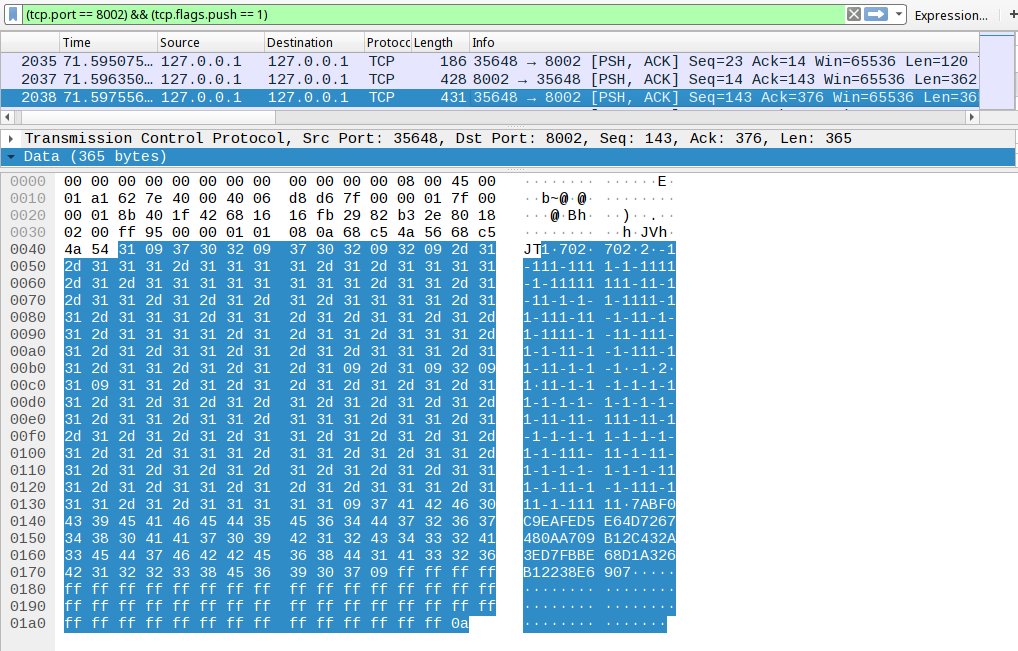
\includegraphics[width=1\textwidth]{Figures/sync7.png}
	\caption[peer message type 1 advanced with processing type 2]{peer message type 1 advanced with processing type 2}
	\label{fig:sync7}
\end{figure}
\FloatBarrier

When this packet arrives at the other peer we can see from the output2 file that the tree parity machine's weights will be updated straight away, unlike last time when the if statement was just skipped.
\begin{lstlisting}
message type 1 receivedwith partner id of 702 and iteration 2

updating machine with this vector 
11-1-1-1-1-1-11-1-1-1-1-1-1-1-1-11-11-111-11-1-1-1-1-11-1-1-1-1-1-111-11-1-11-1-1-1-1-1-1-1-111-1-11-1-1-111-111-1-11111
\end{lstlisting}
This time the code inside here will be executed.
\begin{lstlisting}
if(tell_machine_to_update == 1){
	old_input_vector = parsed_msg.at(8);
	tpm_networks_[index].set_random_input_vector_from_string(old_input_vector);
	if(PRINT_SYNC_MESSAGES){
		std::cout << "\nupdating machine with this vector \n" << old_input_vector << "\n";
	}
	tpm_networks_[index].update_weight();
	
	std::string other_key = parsed_msg.at(9);
	//key = tpm_networks_[index].get_key();
	
	random_input_for_key = parsed_msg.at(10);
	key_hash = parsed_msg.at(9);
	
	std::string key_hash_this = tpm_networks_[index].calc_test(random_input_for_key);

	if (!key_hash.compare(key_hash_this)) {
		// keys are the same
		if(PRINT_SYNC_MESSAGES){
			std::cout << "found same key hash : " << key_hash_this << std::endl;
		}
		tpm_networks_[index].add_key_to_proper_keys(tpm_networks_[index].get_key());
		//std::exit(1);
		
		// reset tpm
		tpm_networks_[index].reset();
		ss << "4\t" << tpm_id << "\t" << tpm_networks_[index].iteration() << "\t" << 0 << "\t" << 1 << "\n";
		//      0       1                   2                                         3            4 //save current key
		return ss.str();
	}
}
\end{lstlisting}
The old vector is set as the input vector and the tree parity machine updates it's weights based on it. Next the new input vector is set and a test is calculated the results of the test is compared to the result of the test sent over the network. If the results are the same then a key has been successfully generated and the tree parity machines are reset. In this case this is not the same so it is skipped and the same bit of code is executed as seen last time. 

The next couple of hundred messages are very similar as they simply synchronise. Currently we are only on sync iteration 2 as seen from the output2 file. Next we will skip all other sync messages until we reach a point where the weights are the same. We can find out roughly where it is in the output files by looking at the tree parity machines logs and looking at the iteration number of when the key was generated.
\begin{figure}[!h]
	\centering
	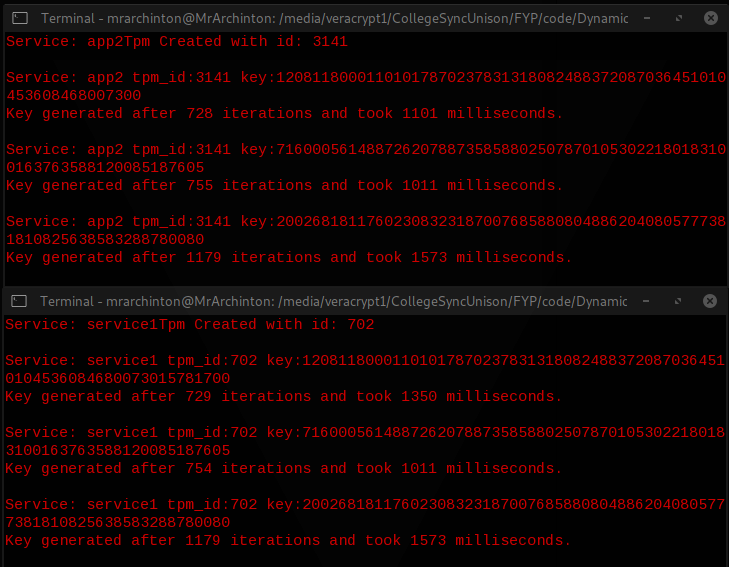
\includegraphics[width=1\textwidth]{Figures/sync11.png}
	\caption[Initial logs of tree parity machines]{Initial logs of tree parity machines}
	\label{fig:sync11}
\end{figure}
\FloatBarrier
As you can see from figure \ref{fig:sync11} where the two terminals are showing the first few lines from the tree parity machines logs. The tree parity machine for service service1 saved the key before the tree parity machine for service app2, after 728 sync iterations and this took 1101 milliseconds to process 728 iterations. The tree parity machine for service app2 received the information to reset due to found key and then checked if the key was actually the same by comparing hashes and since the hashes were the same the key was then saved on the 728th iteration. 

So if we look in the output2 file at iteration 728 we will find the key being saved. Also just a reminder the key you see in the figure is not actually the key that will be used for encryption it is more or less a sequence of numbers that will be used to generate said key. The key displayed here is actually the weights shifted (more on this later). 
\begin{lstlisting}
message type 1 receivedwith partner id of 702 and iteration 728

iteration 728message type: 2tell_machine_to_update 1
key_hashed: 1AD810008E1DA0FE237027BA15FA5998478C9EC30AE799789735B15366CD05BA
old: 1-11-1-1-1-1111-11-1-11-1-111-1-1-1-1-1-1-11-1-11-111-1-1-1-1-11-111111-111-1-11-111-11-111-11-11-1-11-1-111-1-1
new:-1-1-1-11-1-1-1-1-111-1-1111-111-1-11-1-111-1-11-1-11-1-1-1-1-1-1-11111-11-1111-11-11-1-1-11-1-1-1-1111111-1-1-11

on_sync: key_couter=728
message type 4 receivedwith partner id of 702 and iteration 0 and stop tpm 0
adding key to proper keys: 120811800011010178702378313180824883720870364510104536084680073015781700
writing to file
second tpm added key to list 120811800011010178702378313180824883720870364510104536084680073015781700Read random value: 5851956340395214260
random number: 5851956340395214260
sync_tpm_message_one end
on_reset: 1	3141	3141	1	1-1-111-1-1-111-111-1-11-1-1-1-1-1-111-11-1-11-11111-1-11-1-1-1-1-111-111-1-111-11-11-1-1-1-11-11-11-111111-11	1	1
\end{lstlisting}
And here is the output from file output1 for the iteration 728

\begin{lstlisting}
iteration 728message type: 2tell_machine_to_update 0
key_hashed: 2F6A9EF82B2764F74396929DCEE7D76C562F18C00BCB9A14D27FD52296FEA459
old: -11-1-11111-1-1-11-1-1-1-11111-111-1-1-11-11-1-1-11-1-1-1-1-1-1-1-1-1-1-1-1-1-1-11-1111-111-1-11-1-1-1-1-1-1-1-1-1-1-111
new:1-11-1-1-1-1111-11-1-11-1-111-1-1-1-1-1-1-11-1-11-111-1-1-1-1-11-111111-111-1-11-111-11-111-11-11-1-11-1-111-1-1

on_sync: key_couter=727
message type 1 receivedwith partner id of 3141 and iteration 728

updating machine with this vector 
1-11-1-1-1-1111-11-1-11-1-111-1-1-1-1-1-1-11-1-11-111-1-1-1-1-11-111111-111-1-11-111-11-111-11-11-1-11-1-111-1-1
found same key hash : 1AD810008E1DA0FE237027BA15FA5998478C9EC30AE799789735B15366CD05BA
adding key to proper keys: 120811800011010178702378313180824883720870364510104536084680073015781700
writing to file
Read random value: 1393070884901232147
random number: 1393070884901232147
on_sync: key_couter=1
\end{lstlisting}
So here we can see that it was the tree parity machine for service1 that found the key first as can be seen by the line starting with found same key hash this key is then added to the key store and then used by the functions covered in the API section. 

When this key was found the tree parity machine reset its weights in order to generate the next key. Resetting weights is just filling them up with random values. 
Then a reset message is sent with the save key tag on.
\begin{lstlisting}
tpm_networks_[index].reset();
ss << "4\t" << tpm_id << "\t" << tpm_networks_[index].iteration() << "\t" << 0 << "\t" << 1 << "\n";
//      0       1                   2                                         3            4 //save current key
\end{lstlisting}
When the other peer receives this message in the on reset function and if the save key part of the message is set then this logic is performed.
\begin{lstlisting}
if(std::stoi(parsed_msg.at(4)) == 1){
	SingleTpmNetworkHandler *hptr = tpm_handler.get_tpm(tpm_id);
	hptr->add_key_to_proper_keys(hptr->get_key());
	std::cout << "second tpm added key to list " << hptr->get_key();
	//std::exit(1);
} 
tpm_handler.reset_tpm(tpm_index);
tpm_handler.increase_iteration(tpm_id);
\end{lstlisting}
After resetting it is back to synchronising so once again the sync tpm message one function is used.
\begin{lstlisting}
if(tpm_found){
	std::stringstream ss;
	ss << tpm_handler.sync_tpm_message_one(tpm_id);
	std::cout << "on_reset: " << ss.str() << std::endl;
	do_write(ss.str());
}
\end{lstlisting}
And the whole cycle continues all over again until the the NodeJs apps tell the API to stop synchronising. 

Adding the keys to the key store is done by the following function.
\begin{lstlisting}
void SingleTpmNetworkHandler::add_key_to_proper_keys(std::string key){
	std::cout << "adding key to proper keys: " << key << std::endl;
	
	//no need to add to objects storage for now
	//proper_keys.push_back(key);
	
	api_service_data_handler.add_key(service_name_, key);
	
	std::chrono::steady_clock::time_point end = std::chrono::steady_clock::now();
	
	std::chrono::duration<int,std::milli> duration( std::chrono::duration_cast<std::chrono::duration<int,std::milli>>(end-time_sync_start_) ) ;
	
	
	if(PRINT_KEYS_TO_EXTERNAL_GNOME_TERMINAL){
		key_log.open(filename, std::ios::out);
		if (key_log.is_open()){
			std::cout << "writing to file" << std::endl;
			key_log << "Service: " << service_name_ << " tpm_id:" << tpm_id_ << " key:" << key << "\nKey generated after " << iteration_ << " iterations" << " and took " << duration.count() << " milliseconds.\n\n" ;
		}else{
			std::cout << "cant write to file" << std::endl;
		}
		key_log.close();
	}else{
		std::cout << "Service: " << service_name_ << " tpm_id:" << tpm_id_ << " key:" << key << "\n Key generated after " << iteration_ << " iterations" << " and took " << duration.count() << " milliseconds.\n"<< std::endl;
	}
	
	time_sync_start_ = std::chrono::steady_clock::now();
}     
\end{lstlisting}
Firstly this function sends the key to the api service data handler object with the name of the service and the key. Then to know how long it took to generate the key the chrono library is used to get the current time and then the duration. After that the information is written to the terminal or just the standard output depending on which arguments DynamiCrypt was executed with. In this case it was written to the terminal. And finally the timer is started once again to see how long it takes to generate the next key.

\begin{lstlisting}
int API_service_data_handler::add_key(std::string name, std::string key){
	API_data* ptr = get_API_data(name, 0);
	if(ptr != NULL){
		ptr->keys_.push_back(key_store());
		ptr->keys_.back().key = key;
		ptr->keys_.back().uses = 0;
		return 1;
	}
	else{
		return 0;
	}
}
\end{lstlisting}

The add key function inside the api service data handler object simply pushes more data into the key store. 

\section{Sync-server Key Generation Performance}
For this section we will take a look at the performance of the sync-server by looking at how fast it can generate keys on average and how many sync iterations occur per time period. This is a continuation from the previous section as the same tree parity machine logs will be used form before. Each log contains 54 keys that were generated.

Here are the logs in full.

\textbf{Log for tree parity machine for service service1}
\begin{lstlisting}
Service: service1Tpm Created with id: 702

Service: service1 tpm_id:702 key:120811800011010178702378313180824883720870364510104536084680073015781700
Key generated after 729 iterations and took 1350 milliseconds.

Service: service1 tpm_id:702 key:716000561488726207887358588025078701053022180183100163763588120085187605
Key generated after 754 iterations and took 1011 milliseconds.

Service: service1 tpm_id:702 key:200268181176023083231870076858808048862040805777381810825638583288780080
Key generated after 1179 iterations and took 1573 milliseconds.

Service: service1 tpm_id:702 key:807211852273088010123443608150867083181480200645181631807253118616808110
Key generated after 439 iterations and took 582 milliseconds.

Service: service1 tpm_id:702 key:128170885766024502800103448121106800728003805002087360017767201488625782
Key generated after 1349 iterations and took 1805 milliseconds.

Service: service1 tpm_id:702 key:052784042781186081042657214621800850005002761810878768061057080670346023
Key generated after 228 iterations and took 303 milliseconds.

Service: service1 tpm_id:702 key:067010817883282267601860108348030018588870211872764803718400738400010533
Key generated after 503 iterations and took 666 milliseconds.

Service: service1 tpm_id:702 key:783078378104613086816771401700818582006868817018841358803280012158381870
Key generated after 1311 iterations and took 1741 milliseconds.

Service: service1 tpm_id:702 key:060062665007878828716162180358107624878748370820861826088028010748217341
Key generated after 1029 iterations and took 1371 milliseconds.

Service: service1 tpm_id:702 key:381804551814674800684838802028871617646803087076087508445206522808800300
Key generated after 727 iterations and took 970 milliseconds.

Service: service1 tpm_id:702 key:816876008067652100283806104880633610817318710800270160058817638780016740
Key generated after 591 iterations and took 784 milliseconds.

Service: service1 tpm_id:702 key:688140300858185070111848133678640100041115870058886510062004152075081203
Key generated after 211 iterations and took 277 milliseconds.

Service: service1 tpm_id:702 key:806577726032080138186301573800438580404860478041706160583786670600078581
Key generated after 1022 iterations and took 1356 milliseconds.

Service: service1 tpm_id:702 key:702180060508076720851178174788081865007386281001427817168017052081854782
Key generated after 462 iterations and took 610 milliseconds.

Service: service1 tpm_id:702 key:503068064076378380203711028332780680816708002487073418633108602218478831
Key generated after 903 iterations and took 1199 milliseconds.

Service: service1 tpm_id:702 key:781271816885605387625883856105783611883078814732283111532008818187333400
Key generated after 384 iterations and took 508 milliseconds.

Service: service1 tpm_id:702 key:611537808870810730206164128040507221801888183002860086867773847818878187
Key generated after 389 iterations and took 513 milliseconds.

Service: service1 tpm_id:702 key:125008360208688888187481751828727018830174086086308077118372288152205006
Key generated after 1023 iterations and took 1355 milliseconds.

Service: service1 tpm_id:702 key:758137022087828417054401005760030728548088060158812068510361767058585170
Key generated after 956 iterations and took 1263 milliseconds.

Service: service1 tpm_id:702 key:421808458668220877137813877478120780638870782321252658000880802783200008
Key generated after 792 iterations and took 1061 milliseconds.

Service: service1 tpm_id:702 key:871000010375328587082882177506262087070020718510008375704615000383101016
Key generated after 1377 iterations and took 1818 milliseconds.

Service: service1 tpm_id:702 key:848016206810014285886166423100260228002801070220811851177088748621670808
Key generated after 724 iterations and took 963 milliseconds.

Service: service1 tpm_id:702 key:006770073672878015350750008183048560080768840202312608881608874070885067
Key generated after 582 iterations and took 769 milliseconds.

Service: service1 tpm_id:702 key:003863781431701868075058680087371678833222825808184012058034528761407028
Key generated after 593 iterations and took 784 milliseconds.

Service: service1 tpm_id:702 key:088071786604828282050578553085408160281618864001604302075878057468086488
Key generated after 581 iterations and took 767 milliseconds.

Service: service1 tpm_id:702 key:881604358873623650088703044678585808588478020118678806482062707038007883
Key generated after 422 iterations and took 566 milliseconds.

Service: service1 tpm_id:702 key:657070703087768082640687837488003761708101888276100084717705181563810850
Key generated after 732 iterations and took 968 milliseconds.

Service: service1 tpm_id:702 key:771006188140853077021750185023871005808201068578481127188781807826871150
Key generated after 891 iterations and took 1180 milliseconds.

Service: service1 tpm_id:702 key:075032065800740882288216201508753468813808883008118011845346577404280885
Key generated after 549 iterations and took 728 milliseconds.

Service: service1 tpm_id:702 key:318000003368700005186148825405501807263886488038382471770200100350107835
Key generated after 456 iterations and took 607 milliseconds.

Service: service1 tpm_id:702 key:440200067877884156401580405608318810406108017514407378138103160170083672
Key generated after 688 iterations and took 909 milliseconds.

Service: service1 tpm_id:702 key:215306810880621070520827610101777658811203088601057758605080581068280106
Key generated after 1329 iterations and took 1761 milliseconds.

Service: service1 tpm_id:702 key:850018316776008881078427147706820883200022583781812050757652076350150162
Key generated after 909 iterations and took 1203 milliseconds.

Service: service1 tpm_id:702 key:007388126338360866017408628743050586487688873087808450177687005015401188
Key generated after 334 iterations and took 434 milliseconds.

Service: service1 tpm_id:702 key:148871088048301876000584264187407883084576681876308750760610812782407365
Key generated after 354 iterations and took 472 milliseconds.

Service: service1 tpm_id:702 key:631408072858024863880106008887106012614021017008355500818888768054831008
Key generated after 496 iterations and took 657 milliseconds.

Service: service1 tpm_id:702 key:188106200175187721081804315030083802811888804818708180488731703000680486
Key generated after 1158 iterations and took 1537 milliseconds.

Service: service1 tpm_id:702 key:321384208618558088450135387580136774068180782005528274780801487805081678
Key generated after 437 iterations and took 578 milliseconds.

Service: service1 tpm_id:702 key:040872018470467083788754014680078110527281501108067808258004020581700676
Key generated after 1127 iterations and took 1503 milliseconds.

Service: service1 tpm_id:702 key:216587704010110073844108188322511750283181073478750150838500880735130815
Key generated after 1081 iterations and took 1429 milliseconds.

Service: service1 tpm_id:702 key:435787060528026844870156760620750706628003030470668707630603881203760721
Key generated after 775 iterations and took 1027 milliseconds.

Service: service1 tpm_id:702 key:816343005058870441128080071330630051816784805110258888767518008106028167
Key generated after 928 iterations and took 1223 milliseconds.

Service: service1 tpm_id:702 key:780553251678551713283808014872230088582843184063178015310200078807535328
Key generated after 738 iterations and took 981 milliseconds.

Service: service1 tpm_id:702 key:182003317681787202236281078236447600003473658817148813800880831388703710
Key generated after 839 iterations and took 1117 milliseconds.

Service: service1 tpm_id:702 key:035282311078850350780716726100206880110406670072804033600706883307330172
Key generated after 987 iterations and took 1311 milliseconds.

Service: service1 tpm_id:702 key:055088885618423167077877708080736820021787885710748046782330148280804038
Key generated after 601 iterations and took 792 milliseconds.

Service: service1 tpm_id:702 key:007700646088073818601028623874630888740827618657088808805786700471168025
Key generated after 790 iterations and took 1047 milliseconds.

Service: service1 tpm_id:702 key:520117345000852522728480508518876604671000076746000275687008817400162708
Key generated after 1072 iterations and took 1415 milliseconds.

Service: service1 tpm_id:702 key:004682084638005585603347020221436787108155130425101081076677783460007047
Key generated after 805 iterations and took 1066 milliseconds.

Service: service1 tpm_id:702 key:774683885071861022400780060008036023001214830766068074418777287860010113
Key generated after 286 iterations and took 376 milliseconds.

Service: service1 tpm_id:702 key:248860183477187037628017688787334016808388281835883814857878267700683471
Key generated after 1074 iterations and took 1420 milliseconds.

Service: service1 tpm_id:702 key:087020711357081875224811681615108120180118850828081585166800813053008617
Key generated after 1130 iterations and took 1496 milliseconds.

Service: service1 tpm_id:702 key:837707578420204787881621660888714888848456740120412046870703188461812188
Key generated after 584 iterations and took 767 milliseconds.

Service: service1 tpm_id:702 key:087868657056818224686027788004628258430032180675284688210703288788788008
Key generated after 1332 iterations and took 1771 milliseconds.

\end{lstlisting}

\textbf{Log for tree parity machine for service app2}
\begin{lstlisting}
Service: app2Tpm Created with id: 3141

Service: app2 tpm_id:3141 key:12081180001101017870237831318082488372087036451010453608468007300
Key generated after 728 iterations and took 1101 milliseconds.

Service: app2 tpm_id:3141 key:716000561488726207887358588025078701053022180183100163763588120085187605
Key generated after 755 iterations and took 1011 milliseconds.

Service: app2 tpm_id:3141 key:200268181176023083231870076858808048862040805777381810825638583288780080
Key generated after 1179 iterations and took 1573 milliseconds.

Service: app2 tpm_id:3141 key:807211852273088010123443608150867083181480200645181631807253118616808110
Key generated after 438 iterations and took 583 milliseconds.

Service: app2 tpm_id:3141 key:128170885766024502800103448121106800728003805002087360017767201488625782
Key generated after 1349 iterations and took 1805 milliseconds.

Service: app2 tpm_id:3141 key:052784042781186081042657214621800850005002761810878768061057080670346023
Key generated after 228 iterations and took 303 milliseconds.

Service: app2 tpm_id:3141 key:067010817883282267601860108348030018588870211872764803718400738400010533
Key generated after 504 iterations and took 666 milliseconds.

Service: app2 tpm_id:3141 key:783078378104613086816771401700818582006868817018841358803280012158381870
Key generated after 1310 iterations and took 1742 milliseconds.

Service: app2 tpm_id:3141 key:060062665007878828716162180358107624878748370820861826088028010748217341
Key generated after 1030 iterations and took 1370 milliseconds.

Service: app2 tpm_id:3141 key:381804551814674800684838802028871617646803087076087508445206522808800300
Key generated after 726 iterations and took 971 milliseconds.

Service: app2 tpm_id:3141 key:816876008067652100283806104880633610817318710800270160058817638780016740
Key generated after 592 iterations and took 784 milliseconds.

Service: app2 tpm_id:3141 key:688140300858185070111848133678640100041115870058886510062004152075081203
Key generated after 210 iterations and took 278 milliseconds.

Service: app2 tpm_id:3141 key:806577726032080138186301573800438580404860478041706160583786670600078581
Key generated after 1023 iterations and took 1356 milliseconds.

Service: app2 tpm_id:3141 key:702180060508076720851178174788081865007386281001427817168017052081854782
Key generated after 461 iterations and took 611 milliseconds.

Service: app2 tpm_id:3141 key:503068064076378380203711028332780680816708002487073418633108602218478831
Key generated after 904 iterations and took 1199 milliseconds.

Service: app2 tpm_id:3141 key:781271816885605387625883856105783611883078814732283111532008818187333400
Key generated after 383 iterations and took 508 milliseconds.

Service: app2 tpm_id:3141 key:611537808870810730206164128040507221801888183002860086867773847818878187
Key generated after 389 iterations and took 513 milliseconds.

Service: app2 tpm_id:3141 key:125008360208688888187481751828727018830174086086308077118372288152205006
Key generated after 1024 iterations and took 1355 milliseconds.

Service: app2 tpm_id:3141 key:758137022087828417054401005760030728548088060158812068510361767058585170
Key generated after 955 iterations and took 1263 milliseconds.

Service: app2 tpm_id:3141 key:421808458668220877137813877478120780638870782321252658000880802783200008
Key generated after 793 iterations and took 1060 milliseconds.

Service: app2 tpm_id:3141 key:871000010375328587082882177506262087070020718510008375704615000383101016
Key generated after 1376 iterations and took 1818 milliseconds.

Service: app2 tpm_id:3141 key:848016206810014285886166423100260228002801070220811851177088748621670808
Key generated after 725 iterations and took 963 milliseconds.

Service: app2 tpm_id:3141 key:006770073672878015350750008183048560080768840202312608881608874070885067
Key generated after 582 iterations and took 769 milliseconds.

Service: app2 tpm_id:3141 key:003863781431701868075058680087371678833222825808184012058034528761407028
Key generated after 593 iterations and took 784 milliseconds.

Service: app2 tpm_id:3141 key:088071786604828282050578553085408160281618864001604302075878057468086488
Key generated after 580 iterations and took 767 milliseconds.

Service: app2 tpm_id:3141 key:881604358873623650088703044678585808588478020118678806482062707038007883
Key generated after 422 iterations and took 566 milliseconds.

Service: app2 tpm_id:3141 key:657070703087768082640687837488003761708101888276100084717705181563810850
Key generated after 733 iterations and took 968 milliseconds.

Service: app2 tpm_id:3141 key:771006188140853077021750185023871005808201068578481127188781807826871150
Key generated after 890 iterations and took 1181 milliseconds.

Service: app2 tpm_id:3141 key:075032065800740882288216201508753468813808883008118011845346577404280885
Key generated after 550 iterations and took 728 milliseconds.

Service: app2 tpm_id:3141 key:318000003368700005186148825405501807263886488038382471770200100350107835
Key generated after 456 iterations and took 607 milliseconds.

Service: app2 tpm_id:3141 key:440200067877884156401580405608318810406108017514407378138103160170083672
Key generated after 688 iterations and took 909 milliseconds.

Service: app2 tpm_id:3141 key:215306810880621070520827610101777658811203088601057758605080581068280106
Key generated after 1329 iterations and took 1761 milliseconds.

Service: app2 tpm_id:3141 key:850018316776008881078427147706820883200022583781812050757652076350150162
Key generated after 909 iterations and took 1203 milliseconds.

Service: app2 tpm_id:3141 key:007388126338360866017408628743050586487688873087808450177687005015401188
Key generated after 334 iterations and took 434 milliseconds.

Service: app2 tpm_id:3141 key:148871088048301876000584264187407883084576681876308750760610812782407365
Key generated after 354 iterations and took 472 milliseconds.

Service: app2 tpm_id:3141 key:631408072858024863880106008887106012614021017008355500818888768054831008
Key generated after 495 iterations and took 657 milliseconds.

Service: app2 tpm_id:3141 key:188106200175187721081804315030083802811888804818708180488731703000680486
Key generated after 1158 iterations and took 1537 milliseconds.

Service: app2 tpm_id:3141 key:321384208618558088450135387580136774068180782005528274780801487805081678
Key generated after 437 iterations and took 578 milliseconds.

Service: app2 tpm_id:3141 key:040872018470467083788754014680078110527281501108067808258004020581700676
Key generated after 1128 iterations and took 1502 milliseconds.

Service: app2 tpm_id:3141 key:216587704010110073844108188322511750283181073478750150838500880735130815
Key generated after 1080 iterations and took 1430 milliseconds.

Service: app2 tpm_id:3141 key:435787060528026844870156760620750706628003030470668707630603881203760721
Key generated after 775 iterations and took 1027 milliseconds.

Service: app2 tpm_id:3141 key:816343005058870441128080071330630051816784805110258888767518008106028167
Key generated after 928 iterations and took 1223 milliseconds.

Service: app2 tpm_id:3141 key:780553251678551713283808014872230088582843184063178015310200078807535328
Key generated after 739 iterations and took 981 milliseconds.

Service: app2 tpm_id:3141 key:182003317681787202236281078236447600003473658817148813800880831388703710
Key generated after 838 iterations and took 1117 milliseconds.

Service: app2 tpm_id:3141 key:035282311078850350780716726100206880110406670072804033600706883307330172
Key generated after 987 iterations and took 1311 milliseconds.

Service: app2 tpm_id:3141 key:055088885618423167077877708080736820021787885710748046782330148280804038
Key generated after 602 iterations and took 791 milliseconds.

Service: app2 tpm_id:3141 key:007700646088073818601028623874630888740827618657088808805786700471168025
Key generated after 789 iterations and took 1047 milliseconds.

Service: app2 tpm_id:3141 key:520117345000852522728480508518876604671000076746000275687008817400162708
Key generated after 1073 iterations and took 1415 milliseconds.

Service: app2 tpm_id:3141 key:004682084638005585603347020221436787108155130425101081076677783460007047
Key generated after 805 iterations and took 1066 milliseconds.

Service: app2 tpm_id:3141 key:774683885071861022400780060008036023001214830766068074418777287860010113
Key generated after 285 iterations and took 376 milliseconds.

Service: app2 tpm_id:3141 key:248860183477187037628017688787334016808388281835883814857878267700683471
Key generated after 1075 iterations and took 1419 milliseconds.

Service: app2 tpm_id:3141 key:087020711357081875224811681615108120180118850828081585166800813053008617
Key generated after 1130 iterations and took 1496 milliseconds.

Service: app2 tpm_id:3141 key:837707578420204787881621660888714888848456740120412046870703188461812188
Key generated after 583 iterations and took 767 milliseconds.

Service: app2 tpm_id:3141 key:087868657056818224686027788004628258430032180675284688210703288788788008
Key generated after 1332 iterations and took 1771 milliseconds.

\end{lstlisting}

Here are the logs with only the important information relating to performance.

\textbf{For service service1 tree parity machine.}
\begin{lstlisting}
 729 iterations , 1350 milliseconds.
754 iterations , 1011 milliseconds.
1179 iterations , 1573 milliseconds.
439 iterations , 582 milliseconds.
1349 iterations , 1805 milliseconds.
228 iterations , 303 milliseconds.
503 iterations , 666 milliseconds.
1311 iterations , 1741 milliseconds.
1029 iterations , 1371 milliseconds.
727 iterations , 970 milliseconds.
591 iterations , 784 milliseconds.
211 iterations , 277 milliseconds.
1022 iterations , 1356 milliseconds.
462 iterations , 610 milliseconds.
903 iterations , 1199 milliseconds.
384 iterations , 508 milliseconds.
389 iterations , 513 milliseconds.
1023 iterations , 1355 milliseconds.
956 iterations , 1263 milliseconds.
792 iterations , 1061 milliseconds.
1377 iterations , 1818 milliseconds.
724 iterations , 963 milliseconds.
582 iterations , 769 milliseconds.
593 iterations , 784 milliseconds.
581 iterations , 767 milliseconds.
422 iterations , 566 milliseconds.
732 iterations , 968 milliseconds.
891 iterations , 1180 milliseconds.
549 iterations , 728 milliseconds.
456 iterations , 607 milliseconds.
688 iterations , 909 milliseconds.
1329 iterations , 1761 milliseconds.
909 iterations , 1203 milliseconds.
334 iterations , 434 milliseconds.
354 iterations , 472 milliseconds.
496 iterations , 657 milliseconds.
1158 iterations , 1537 milliseconds.
437 iterations , 578 milliseconds.
1127 iterations , 1503 milliseconds.
1081 iterations , 1429 milliseconds.
775 iterations , 1027 milliseconds.
928 iterations , 1223 milliseconds.
738 iterations , 981 milliseconds.
839 iterations , 1117 milliseconds.
987 iterations , 1311 milliseconds.
601 iterations , 792 milliseconds.
790 iterations , 1047 milliseconds.
1072 iterations , 1415 milliseconds.
805 iterations , 1066 milliseconds.
286 iterations , 376 milliseconds.
1074 iterations , 1420 milliseconds.
1130 iterations , 1496 milliseconds.
584 iterations , 767 milliseconds.
1332 iterations , 1771 milliseconds.

\end{lstlisting}

\textbf{For service app2 tree parity machine.}
\begin{lstlisting}
 728 iterations , 1101 milliseconds.
755 iterations , 1011 milliseconds.
1179 iterations , 1573 milliseconds.
438 iterations , 583 milliseconds.
1349 iterations , 1805 milliseconds.
228 iterations , 303 milliseconds.
504 iterations , 666 milliseconds.
1310 iterations , 1742 milliseconds.
1030 iterations , 1370 milliseconds.
726 iterations , 971 milliseconds.
592 iterations , 784 milliseconds.
210 iterations , 278 milliseconds.
1023 iterations , 1356 milliseconds.
461 iterations , 611 milliseconds.
904 iterations , 1199 milliseconds.
383 iterations , 508 milliseconds.
389 iterations , 513 milliseconds.
1024 iterations , 1355 milliseconds.
955 iterations , 1263 milliseconds.
793 iterations , 1060 milliseconds.
1376 iterations , 1818 milliseconds.
725 iterations , 963 milliseconds.
582 iterations , 769 milliseconds.
593 iterations , 784 milliseconds.
580 iterations , 767 milliseconds.
422 iterations , 566 milliseconds.
733 iterations , 968 milliseconds.
890 iterations , 1181 milliseconds.
550 iterations , 728 milliseconds.
456 iterations , 607 milliseconds.
688 iterations , 909 milliseconds.
1329 iterations , 1761 milliseconds.
909 iterations , 1203 milliseconds.
334 iterations , 434 milliseconds.
354 iterations , 472 milliseconds.
495 iterations , 657 milliseconds.
1158 iterations , 1537 milliseconds.
437 iterations , 578 milliseconds.
1128 iterations , 1502 milliseconds.
1080 iterations , 1430 milliseconds.
775 iterations , 1027 milliseconds.
928 iterations , 1223 milliseconds.
739 iterations , 981 milliseconds.
838 iterations , 1117 milliseconds.
987 iterations , 1311 milliseconds.
602 iterations , 791 milliseconds.
789 iterations , 1047 milliseconds.
1073 iterations , 1415 milliseconds.
805 iterations , 1066 milliseconds.
285 iterations , 376 milliseconds.
1075 iterations , 1419 milliseconds.
1130 iterations , 1496 milliseconds.
583 iterations , 767 milliseconds.
1332 iterations , 1771 milliseconds.

\end{lstlisting}

In order to perform calculations this data will be read into a python program. Here is the python script used. Matplotlib is used to create the graphs.

\begin{lstlisting}
#!/usr/bin/env python3.7

import matplotlib.pyplot as plt

service1_iterations = []
service1_time = []

app2_iterations = []
app2_time = []

with open("./keys_service1_short") as f:
	for line in f:
		service1_iterations.append(int(line.split()[0]))
		service1_time.append(int(line.split()[3]))
		#print(line.split()[3])


with open("./keys_app2_short") as f:
	for line in f:
		app2_iterations.append(int(line.split()[0]))
		app2_time.append(int(line.split()[3]))
		#print(line.split()[3])


service1_iterations_total = 0
service1_time_total = 0

app2_iterations_total = 0
app2_time_total = 0

for item in service1_iterations:
	service1_iterations_total = service1_iterations_total + item

for item in service1_time:
	service1_time_total = service1_time_total + item

for item in app2_iterations:
	app2_iterations_total = app2_iterations_total + item

for item in app2_time:
	app2_time_total = app2_time_total + item		


print("total iterations for service1 = ", service1_iterations_total)
print("total time for service1 = ", service1_time_total, " milliseconds ")
print("total iterations for app2 = ", app2_iterations_total)
print("total time for app2 = ", app2_time_total, " milliseconds \n")
#print(service1_iterations)

print("iterations per second for service1 = ", (service1_iterations_total / service1_time_total)*1000)
print("iterations per second for app2 = ", (app2_iterations_total / app2_time_total)*1000)

plt.plot(service1_iterations, service1_time, color="green", linewidth=2.5)
plt.xlabel('iterations')
plt.ylabel('time ms')
plt.title('Service1')
plt.show()


plt.plot(app2_iterations, app2_time, color="green", linewidth=2.5)
plt.xlabel('iterations')
plt.ylabel('time ms')
plt.title('App2')
plt.show()
\end{lstlisting}
The output of running this script is seen in figure \ref{fig:sync12}

\begin{figure}[!h]
	\centering
	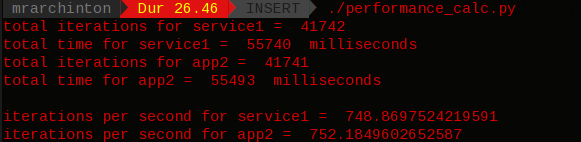
\includegraphics[width=1\textwidth]{Figures/sync12.png}
	\caption[Output of python script]{Output of python script}
	\label{fig:sync12}
\end{figure}
\FloatBarrier
From the output we can see that after generating 54 keys the total amount of sync iterations performed was 41742 by the peer handling service service1 and 41741 by the peer handling service app2. 

The iteration count here is off by one which is what is expected and therefore we can say that the system worked well.

It took the tree parity machine for service service1 55740 milliseconds or 55.74 seconds to generate 54 keys. The tree parity machine for service app2 was a little bit faster and generated those 54 keys in 55493 milliseconds or 55.49 seconds. 

Again the total time it took to generate the 54 keys is only off by 0.247 seconds this is perfectly ok also since the network can be unpredictable if there are other apps and servers accessing it. In this case there were a number of local host clients and apps so this result is very reasonable.

The final calculation is the average number of iterations that can be processed by the tree parity machines.

The tree parity machine for service service1 averages around 749 sync iterations per second. The tree parity machine for service app2 averages around 752 sync iterations per second. 

Once again this is a very close result and considering how fast they synchronise this is perfectly acceptable. Since app2 was using a listening peer instead of a connecting peer like service1 this will result in a few less iterations because of the way the reset function handles the iteration counts and it is normally the connecting peer's tree parity machines that find the key.

The last part is to see how stable the sync-server is so the number of iterations will be plotted in a line graph against the equivalent time it took to perform all of those iterations. For a stable system the line should be fairly straight so the lower number of iterations the faster it should take. 

Figures \ref{fig:sync_results_graph_service1} and \ref{fig:sync_results_graph_app2} show the graphs described.

\begin{figure}[!h]
	\centering
	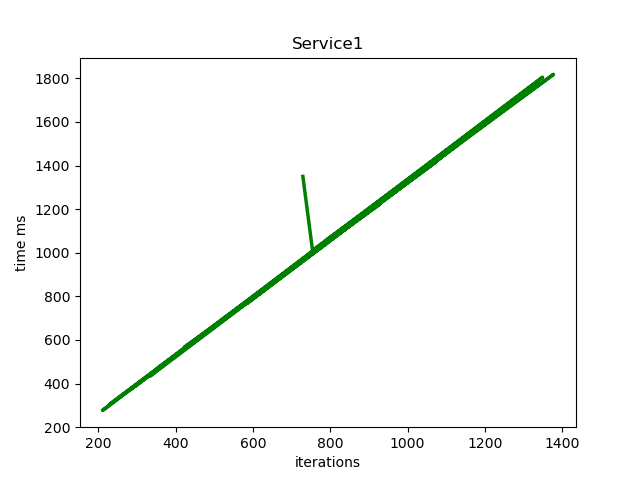
\includegraphics[width=1\textwidth]{Figures/sync_results_graph_service1.png}
	\caption[Graph of iterations against time for service1 tree parity machine]{Graph of iterations against time for service1 tree parity machine}
	\label{fig:sync_results_graph_service1}
\end{figure}
\FloatBarrier

\begin{figure}[!h]
	\centering
	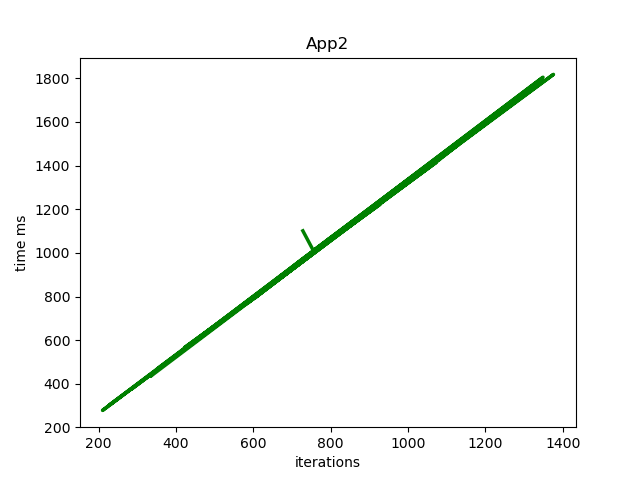
\includegraphics[width=1\textwidth]{Figures/sync_results_graph_app2.png}
	\caption[Graph of iterations against time for app2 tree parity machine]{Graph of iterations against time for app2 tree parity machine}
	\label{fig:sync_results_graph_app2}
\end{figure}
\FloatBarrier

From the diagrams you can see that both have a very straight line apart from one point just before the 800 iteration count. For figure \ref{fig:sync_results_graph_service1} this is more pronounced. This is actually the result for the first key generated by both as can be seen in figure \ref{fig:sync13} which is a screen shot from the top of the tree parity machine log files.

\begin{figure}[!h]
	\centering
	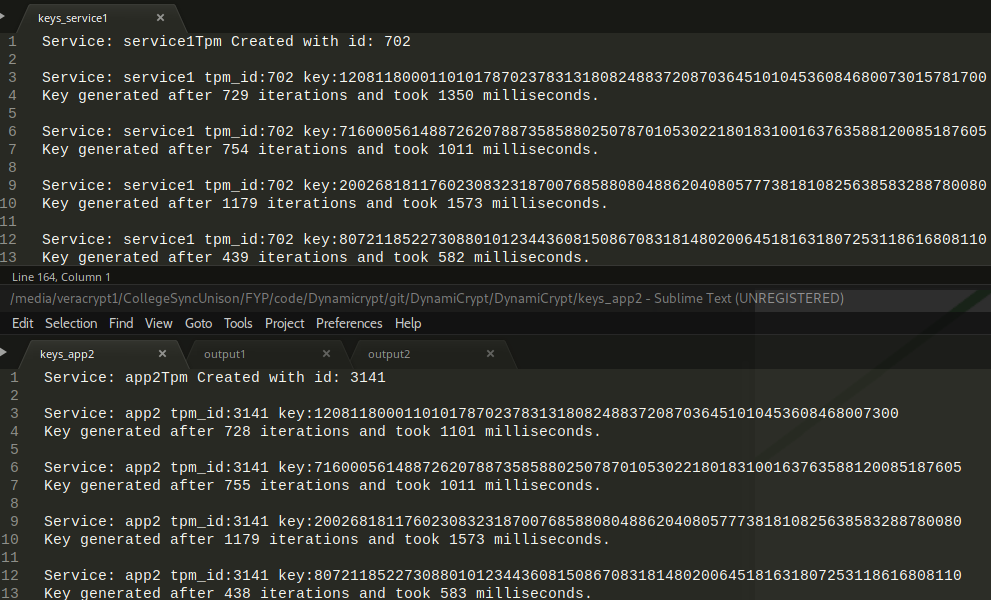
\includegraphics[width=1\textwidth]{Figures/sync13.png}
	\caption[Beginning of tree parity machine logs]{Beginning of tree parity machine logs}
	\label{fig:sync13}
\end{figure}
\FloatBarrier

The reason the first key timer is noticeably longer than the other is because in order to make the timer work properly for all of the other keys, the timer for the first key is started in the constructor of the SingleTpmNetworkHander object. Since the constructor then goes about creating the actual tree parity machine followed by setting up the tree parity machines to communicate with each other by going through the linking function and so on, the time it takes to finally synchronise the key is obviously longer compared to when after the first key the peers only really use sync messages and reset but reset just generates sync messages anyway. 

Therefore this can be considered as a false positive and therefore ignored. From the graphs then we can see that the sync-server of DynamiCrypt is very stable and there is no decline in performance when it processes either 1400 iterations for one key or 200 iterations for one key.

All of these logs and the python script are available in the GitHub repository in the following location:
\begin{lstlisting}
DynamiCrypt/thesis_logs_and_scripts/
\end{lstlisting}
%\begin{lstlisting}
%\end{lstlisting}
%tree parity machine
%\begin{figure}[!h]
%\centering
%	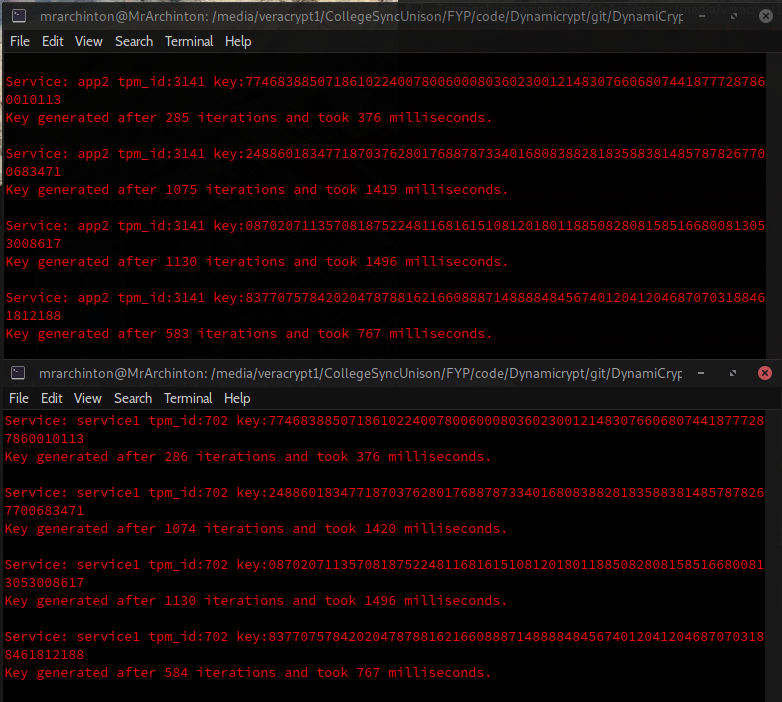
\includegraphics[width=1\textwidth]{Figures/sync2.png}
%	\caption[Ending of tree parity machine logs]{Ending of tree parity machine logs}
%	\label{fig:sync2}
%\end{figure}
%\FloatBarrier